\documentclass{article}

%\documentclass[twocolumn]{article}
%\documentclass{book}
\usepackage{parskip}
\usepackage[bottom=1in]{geometry}
\usepackage{multicol}
\setlength{\columnsep}{0.9cm}
\usepackage{supertabular}
\usepackage[utf8]{inputenc}
%\usepackage{geometry}   % Setup for page and paper dimensions
\usepackage{wrapfig}
\usepackage{subfigure}
\usepackage{caption}
\captionsetup{
  font=small,
  labelfont=bf,
  tableposition=top
}
\usepackage{float}
\usepackage[swedish,english]{babel}
\usepackage{hyperref}
\hypersetup{
    colorlinks,
    citecolor=black,
    filecolor=black,
    linkcolor=black,
    urlcolor=black,
    pdfborder = {0 0 0}
}
\usepackage{enumitem}
\usepackage{verbatimbox}
\usepackage{fancyvrb}
\usepackage{graphicx}   
\usepackage{lipsum}  
\usepackage[leqno]{amsmath}
\usepackage{listings} 
\usepackage{tikz}
\usepackage{cancel}
\usepackage{steinmetz}
\usepackage{boxdims}

\newcommand*\mycirc[1]{%
\begin{tikzpicture}[baseline={(0,-0.1)}]
\node[draw,circle,inner sep=1pt] {#1};
\end{tikzpicture}}

\newcommand*\textcircle[1]{\textcircled{\raisebox{0.14em}{#1}}}
\newcommand{\quotes}[1]{``#1''}
\usepackage{ifthen}

\makeatletter
\newcommand*{\rom}[1]{\expandafter\@slowromancap\romannumeral #1@}
\makeatother

\usepackage{graphicx}

\makeatletter
\newcommand*\bigcdot{\mathpalette\bigcdot@{.5}}
\newcommand*\bigcdot@[2]{\mathbin{\vcenter{\hbox{\scalebox{#2}{$\m@th#1\bullet$}}}}}
\makeatother

\setlength{\parindent}{0pt}

\newcommand*\sepline{%
  \begin{center}
    \rule[1ex]{.5\textwidth}{.5pt}
  \end{center}}

\newcommand*\sepstars{%
  \begin{center}
    $\star\star\star$
  \end{center}}

\title{Lab RF\\}
\author{Lasse Karagiannis}
\date{\today} % Activate to display a given date or no date (if empty),
         % otherwise the current date is printed 
         
\mathchardef\mhyphen="2D

\usepackage{silence}
\WarningFilter{latex}{Underfull}
\WarningFilter{latex}{Overfull}
\WarningFilter{latex}{Text page}
\usepackage{subfiles}



\usepackage{tikz}
\usepackage{tikz}
\usepackage{pgfplots}
\usepgfplotslibrary{smithchart}
\pgfplotsset{compat=1.11}

\newcommand\mtotex[2]{\immediate\write18{m4 #2.m4 | dpic -#1 > #2.tex}}

\begin{filecontents}[overwrite,noheader,nosearch]{sample1.m4}
%\begin{filecontents*}[noheader,force]{sample1.m4}
include(pgf.m4)
.PS
cct_init
elen = 0.75
Origin: Here
source(up_ elen); llabel(-,v_s,+)
resistor(right_ elen); rlabel(,R,)
dot
{  
capacitor(down_ to (Here,Origin))
rlabel(+,v,-);llabel(,C,)
dot
}
line right_ elen*3/3
inductor(down_ Here.y-Origin.y); rlabel(,L,);b_current(i)
line to Origin
.PE
\end{filecontents}

\begin{filecontents}[overwrite,noheader,nosearch]{sample2.m4}
%\begin{filecontents*}[noheader,force]{sample1.m4}
include(pgf.m4)
.PS
cct_init
elen = 0.75
Origin: Here
source(up_ elen,AC); llabel(-,v_s,+)
resistor(right_ elen); rlabel(,R,)
dot
{  

dot
}
line right_ elen*3/3
resistor(down_ Here.y-Origin.y); rlabel(,R,);

line left_ elen*3/3
dot
line to Origin
.PE
\end{filecontents}



\begin{filecontents}[overwrite,noheader,nosearch]{sample3.m4}
%\begin{filecontents*}[noheader,force]{sample1.m4}
include(pgf.m4)
.PS
cct_init
elen = 0.75
Origin: Here
source(up_ elen,AC); llabel(-,v_s,+)
resistor(right_ elen); rlabel(,R,)
dot
{  

dot
}
line right_ elen*1/3
tline(right_ elen);rlabel(,T-line,)
line right_ elen*1/3
dot
line right_ elen*1/3
resistor(down_ Here.y-Origin.y); rlabel(,R,);label(,25,);

line left_ elen*1/3
dot
line left_ elen*5/3
dot
line to Origin
.PE
\end{filecontents}


\begin{filecontents}[overwrite,noheader,nosearch]{sample3A.m4}
include(pgf.m4)
.PS
cct_init
elen = 0.75
Vs: source(up_ elen,AC); llabel(-,v_s,+)
resistor(right_ elen); rlabel(,R_g`\,'50\Omega,) # rlabel sets math mode
D1: dot
#{
#
#dot
#}
line right_ elen*1/3
tline(right_ elen);rlabel(,\hbox{\sl T-line}`\,'50\Omega,)
line right_ elen*1/3
D2: dot
line right_ elen*1/3
resistor(down_ Here.y-Origin.y); rlabel(,R_L,);llabel(,25\Omega,);

#line left_ elen*1/3
#dot
{ dot(at (D1,Here)) }
{ dot(at (D2,Here)) }
#line left_ elen*5/3
line to Vs.start
.PE
\end{filecontents}

\begin{document}

\begin{titlepage}
\maketitle
\end{titlepage}
\tableofcontents
\vfill\null
\newpage

%\mtotex{g}{sample1}
%\par
%\begin{figure}[ht]
%%\begin{filecontents*}[noheader,force]{sample1.m4}

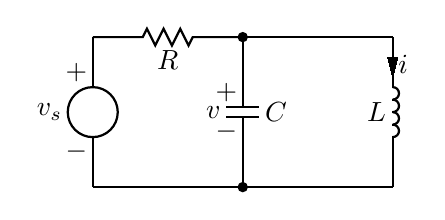
\begin{tikzpicture}[scale=2.54]
% dpic version 2014.Jan.01 option -g for TikZ and PGF 1.01
\ifx\dpiclw\undefined\newdimen\dpiclw\fi
\global\def\dpicdraw{\draw[line width=\dpiclw]}
\global\def\dpicstop{;}
\dpiclw=0.8bp
\dpiclw=0.8bp
\dpicdraw (0,0)
 --(0,0.25)\dpicstop
\dpicdraw (0,0.375) circle (0.049213in)\dpicstop
\dpicdraw (0,0.5)
 --(0,0.75)\dpicstop
\draw (0,0.25) node[below left=-1.5bp]{$ -$};
\draw (-0.125,0.375) node[left=-1.5bp]{$ v_s$};
\draw (0,0.5) node[above left=-1.5bp]{$ +$};
\dpicdraw (0,0.75)
 --(0.25,0.75)
 --(0.270833,0.791667)
 --(0.3125,0.708333)
 --(0.354167,0.791667)
 --(0.395833,0.708333)
 --(0.4375,0.791667)
 --(0.479167,0.708333)
 --(0.5,0.75)
 --(0.75,0.75)\dpicstop
\draw (0.375,0.708333) node[below=-1.5bp]{$ R$};
\dpicdraw[fill=black](0.75,0.75) circle (0.007874in)\dpicstop
\dpicdraw (0.75,0.75)
 --(0.75,0.4)\dpicstop
\dpicdraw (0.666667,0.4)
 --(0.833333,0.4)\dpicstop
\dpicdraw (0.666667,0.35)
 --(0.833333,0.35)\dpicstop
\dpicdraw (0.75,0.35)
 --(0.75,0)\dpicstop
\draw (0.75,0.4) node[above left=-1.5bp]{$ +$};
\draw (0.666667,0.375) node[left=-1.5bp]{$ v$};
\draw (0.75,0.35) node[below left=-1.5bp]{$ -$};
\draw (0.833333,0.375) node[right=-1.5bp]{$ C$};
\dpicdraw[fill=black](0.75,0) circle (0.007874in)\dpicstop
\dpicdraw (0.75,0.75)
 --(1.5,0.75)\dpicstop
\dpicdraw (1.5,0.75)
 --(1.5,0.5)\dpicstop
\dpicdraw (1.5,0.5)
 --(1.494444,0.5)\dpicstop
\dpicdraw (1.5,0.5)
 ..controls (1.517259,0.5) and (1.53125,0.486009)
 ..(1.53125,0.46875)
 ..controls (1.53125,0.451491) and (1.517259,0.4375)
 ..(1.5,0.4375)\dpicstop
\dpicdraw (1.5,0.4375)
 --(1.494444,0.4375)\dpicstop
\dpicdraw (1.5,0.4375)
 ..controls (1.517259,0.4375) and (1.53125,0.423509)
 ..(1.53125,0.40625)
 ..controls (1.53125,0.388991) and (1.517259,0.375)
 ..(1.5,0.375)\dpicstop
\dpicdraw (1.5,0.375)
 --(1.494444,0.375)\dpicstop
\dpicdraw (1.5,0.375)
 ..controls (1.517259,0.375) and (1.53125,0.361009)
 ..(1.53125,0.34375)
 ..controls (1.53125,0.326491) and (1.517259,0.3125)
 ..(1.5,0.3125)\dpicstop
\dpicdraw (1.5,0.3125)
 --(1.494444,0.3125)\dpicstop
\dpicdraw (1.5,0.3125)
 ..controls (1.517259,0.3125) and (1.53125,0.298509)
 ..(1.53125,0.28125)
 ..controls (1.53125,0.263991) and (1.517259,0.25)
 ..(1.5,0.25)\dpicstop
\dpicdraw (1.5,0.25)
 --(1.494444,0.25)\dpicstop
\dpicdraw (1.5,0.25)
 --(1.5,0)\dpicstop
\draw (1.494444,0.375) node[left=-1.5bp]{$ L$};
\filldraw[line width=0bp](1.475,0.65)
 --(1.5,0.55)
 --(1.525,0.65) --cycle
\dpicstop
\dpicdraw (1.5,0.572906)
 --(1.5,0.65)\dpicstop
\draw (1.5,0.611453) node[right=-1.5bp]{$ i$};
\dpicdraw (1.5,0)
 --(0,0)\dpicstop
\end{tikzpicture}

%\caption{customized caption}
%\label{Symbolic_label}
%\end{figure}



%\begin{tikzpicture}
%        \begin{smithchart}
%        \path[draw=red] (0pt,0pt) circle (1.5cm);
%        \path[draw=blue] (0.1,0.5) circle (0.75cm);
%        \path[draw=blue,fill=blue] (0.1,0.5) circle (0.05cm);
%
%       \addplot coordinates {(0.5,0.2) (1,0.8) (2,2)};
%        \end{smithchart}
%    \end{tikzpicture}

\section{Summary}
We designed two solid state microwave amplifiers where one was optimized for maximum gain
and the other was en LNA of gain 13 dB and 1.96 dB Noise figure.
We didn't use Pozar fro the specific gain design but found a book on-line by Orfanidis
``Electromagnetic Waves \& Antennas'' who provided a clear description of how to
proceed without the uilateral assumption ad who also provided a Matlab-toolbox which
could be used with Octave. 
Adapting his examples to a different S-parameter first for the specific gain and
then for smallest possible noise figure was straightforward.

With the correct values for line lengths and stub lengths S-parameter sweeps
were done in QUCS

Realization of the design was done at Uppsala Uiversity with FR4 board ad copper tape
as mirostrip lines.

The measured results differed sigificantly to the simulated results, the optimal bias point
was 3.01V compared to 6V which is what was prescribed i the S-parameter data file.

\section{Design for maximum gain}
\begin{multicols}{2}

We know that for maximum power transfer
$\Gamma_{in}^* = \Gamma_S$ and $\Gamma_{out}^*=\Gamma_L$

\begin{flalign*}
G_{TU}&=\underbrace{\frac{1-|\Gamma_S|^2}{|1-\Gamma_S\Gamma_{in}|^2}}_{G_S}\cdot \underbrace{|S_{21}|^2}_{G_0} \cdot \underbrace{\frac{1-|\Gamma_L|^2}{|1-S_{22}\Gamma_L|^2}}_{G_L}\\
      &=\underbrace{\frac{1-|\Gamma_S|^2}{|1-|\Gamma_S|^2|^2}}_{G_S}\cdot \underbrace{|S_{21}|^2}_{G_0} \cdot \underbrace{\frac{1-|\Gamma_L|^2}{|1-S_{22}\Gamma_L|^2}}_{G_L}\\
\end{flalign*}
Up and down factors cancels and we get
\begin{flalign*}
G_{TU}&=\underbrace{\frac{1}{|1-|\Gamma_S|^2|}}_{G_S}\cdot \underbrace{|S_{21}|^2}_{G_0} \cdot \underbrace{\frac{1-|\Gamma_L|^2}{|1-S_{22}\Gamma_L|^2}}_{G_L}\\
\end{flalign*}
To achive this we solve
\begin{flalign*}
\Gamma_S^*=\Gamma_{in}&=S_{11} +\frac{S_{12} S_{21}\Gamma_L}{1 - S_{22}\Gamma_L}\\
\Gamma_L^*=\Gamma_{out}&=S_{22}+\frac{S_{12}S_{21}\Gamma_S}{1-S_{11}\Gamma_S}\\
\end{flalign*}
which gives the solutions
\begin{flalign*}
\Gamma_S &=\frac{B_1\pm \sqrt{B_1^2-4|C_1|}}{2C_1}\\
         &\text{ where}\\
B_1 &= 1+ |S_{11}|^2-|S_{22}|^2 - \Delta\\
C_1 &= S_{11}- \Delta \cdot S_{22}^*
\end{flalign*}
and $\Gamma_L$ is given by
\begin{flalign*}
\Gamma_L &=\frac{B_2\pm \sqrt{B_2^2-4|C_2|}}{2C_2}\\
         &\text{ where}\\
B_2 &= 1+ |S_{22}|^2-|S_{11}|^2 - \Delta\\
C_2 &= S_{22}- \Delta \cdot S_{11}^*
\end{flalign*}
We are requested to provide a design for 2.45GHz but we don't have
S-parameters for that frequecy so we decided on 2.4 GHz and hoping that the
design would have enough bandwidth.
For the desing we used Octave and verified each step with a Matlab library\footnote{\url{http://eceweb1.rutgers.edu/~orfanidi/ewa/}}
\begin{verbatim}
clear all
% addpath("/home/lasse/ewa")
%Add above statement to console input
i=sqrt(-1);
disp("S-Params at 1.8GHz BFG520 ...
       Common Emitter 6V10mA")
S11_r = 0.494
Theta_S11_grad=166
S21_r=3.722
Theta_S21_grad=74.3
S12_r=0.082
Theta_S12_grad= 56.4
S22_r=0.317
Theta_S22_grad= -57.9
%Call to the EMW-library
disp("")
S=smat([0.494 166.0 3.722 74.3 0.082 ...
     56.4 0.317 -57.9 ])
disp("")
\end{verbatim}
We convert to cartesian coordinates, not shown here, but the full program will in the appendix
We did the Rollet-stability test
\begin{verbatim}
%Stability check
disp('Stability check')
Delta = S11*S22-S12*S21
K_Stab=(1-abs(S11)^2-abs(S22)^2+abs(Delta)^2)...
      /(2*abs(S12*S21))
Abs_Delta = abs(Delta)
if(K_Stab>1 & Abs_Delta<1)
 disp("Stability OK")
else
 disp("Stability not OK")
end
\end{verbatim}
Which resulted in $K = 1.1220$ and $|\Delta|= 0.175$ which means that it stable at the frequecy though unstable
at lower frequencies as previously shown.
Stability circles using the toolbox are
using commands
\begin{verbatim}
[cL,rL] = sgcirc(S,'l');
[cG,rG] = sgcirc(S,'s'); 
smith;
smithcir(cL, rL, 1.1, 1.5);
smithcir(cG, rG, 1.1, 1.5);
\end{verbatim}
Unfourtunately the toolbox doesn't seem to give the option to insert a legend but the upper is the load stability circle
and the lower is the source stability cirlce. They are both outside the unit circle and this means
that any source and load impedances will not result in instability.
\begin{figure}[H]
  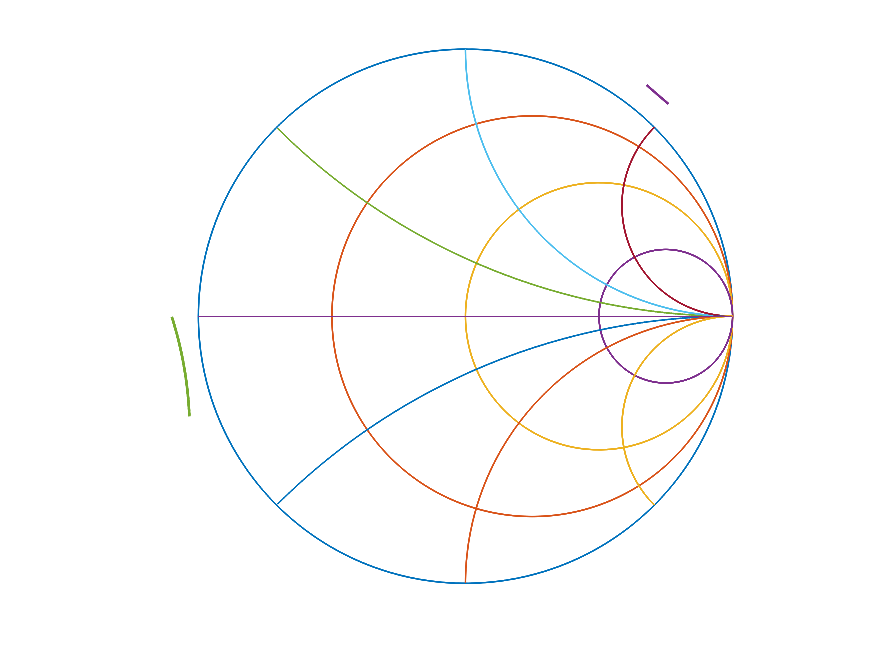
\includegraphics[width=\linewidth]{stability.png}
  \caption{Load stabilty circle (upper). Source stability circle (lower)}
  \label{fig4}
\end{figure}
We calculated to source and load reflection coefficients $\Gamma_s$ and $\Gamma_L$
for a conjugate match which means $\Gamma_s^* = \Gamma_{in}$ and $\Gamma_L^*= \Gamma_{out}$.

\begin{verbatim}
%Maximum gain calculations
disp("Maximum gain calculations")
B1=1+abs(S11)^2-abs(S22)^2 -abs(Delta)^2
B2=1+abs(S22)^2-abs(S11)^2 -abs(Delta)^2
C1=S11 - Delta*conj(S22)
C2=S22 - Delta*conj(S11)
disp("")
%Library calculation
[K,mu,D,B1,B2,C1,C2,D1,D2] = sparam(S)
disp("")


Gamma_S_plus  = (B1 + sqrt(B1^2 
               -4*abs(C1)^2) )/(2*C1);
Gamma_S_minus = (B1 - sqrt(B1^2 
               -4*abs(C1)^2) )/(2*C1);
if(abs(Gamma_S_plus)<1)
  Gamma_MS=Gamma_S_plus
  disp("Returned Gamma_S_plus")
else
  Gamma_MS=Gamma_S_minus
  disp("Returned Gamma_S_minus")
endif

Gamma_L_plus  = (B2 + sqrt(B2^2 ....
               -4*abs(C2)^2) )/(2*C2);
Gamma_L_minus = (B2 - sqrt(B2^2....
               -4*abs(C2)^2) )/(2*C2);
if(abs(Gamma_L_plus)<1)
  Gamma_ML=Gamma_L_plus
  disp("Returned Gamma_L_plus")
else
  Gamma_ML=Gamma_L_minus
  disp("Returned Gamma_L_minus")
endif
\end{verbatim}
In all situations when we tested different S-parameters to learn we always
for some reason had to pick the value which was calculated
with the minus sign before the square root.
Our Octave print-out was the following
\begin{verbatim}
Gamma_MS = -0.7395 - 0.1306i
Gamma_ML =  0.4402 + 0.5100i

AbsGamma_MS = 0.7510
Theta_deg = -169.99
AbsGamma_ML = 0.6737
Theta_deg = 49.204

Gammas according to Matlab toolbox
Gamma_S_Match = -0.7395 - 0.1306i
Gamma_L_Match =  0.4402 + 0.5100i
\end{verbatim}
Matching is simply done by plotting the corresponding impedance on the smith chart
and transforming it to the load impedance/generator impedance, in this case 50 Ohm, but always walk ``towards the load''.
Everything works precisely the same for as for single stub matching of a 50 Ohm line when you walk ``towards the generator''
but here instead you walk ``towards the load''.

We calculated the tranceducer gain $G_T$ correct, in agreement witht the toolbox result
but could not get the correct result for for the operating power gain $G$ and the availibe power gain $G_A$.
\begin{verbatim}
%Gains of matching networks
disp("Gains of matching networks")
%Gain source matching network
G_S=1/(1-abs(Gamma_MS)^2)
G_S_dB=10*log10(G_S)
%Intrinsic gain
G_0=abs(S21)^2
G_0_dB=10*log10(G_0)
%Gain load matching network
G_L=(1-abs(Gamma_ML)^2)...
       /(abs(1-S22*Gamma_ML)^2)
G_L_dB=10*log10(G_L)
disp("Gt gain")
Gt = G_0*G_S*G_L
Gt_dB = G_S_dB+G_0_dB+G_L_dB
Gamma_L_unmatched =0;%no-conjugate match
%Power gain
%Source conj. matched but not the load
G_power=(1/(1-abs(Gamma_MS)^2))*abs(S21)^2...
    *((1-abs(Gamma_L_unmatched)^2)...
     /(abs(1-S22*Gamma_L_unmatched)^2))
G_power_dB=10*log10(G_power)
%Availible power gain
%Load is conj.matched but not source
Gamma_G_unmatched=0
G_availible=((1-abs(Gamma_G_unmatched)^2)...
    /(abs(1-S11*Gamma_G_unmatched)^2))...
    *(abs(S21)^2)*(1/(1-abs(Gamma_ML)^2))
G_availible_dB=10*log10(G_availible)
\end{verbatim}
The print out was the following ommitting unneccesary data
\begin{verbatim}

Gains of matching networks
G_S_dB = 3.6047
G_0_dB = 11.416
G_L_dB = -0.5749
Gt_dB = 14.445
G_power_dB = 15.020
G_availible_dB = 14.043

Gains from toolbox
transducer power gain 
   at given optimized GammmaG and GammaL
Gt_dB = 14.445
available power gain at
   given GammaG with GammaL = GammaOut*
Ga_dB = 11.875
operating power gain 
     at given GammaL with GammaG = GammaIn*
Gp_dB = 12.631
maximum unilateral gain
Gu_dB = 13.090
maximum available gain (MAG)
Gmag_dB = 14.445
maximum stable gain (MSG)
Gmsg_dB = 16.570
\end{verbatim}
I have not understood the gains correctly reagarding 
how to calculate them.
The input and output stubs and the corresponding
serial lines were calculated through the toolbox
\begin{verbatim}
disp("Stubs")
dl_in = stub1 (conj(z_S) ,'po')
dl_out = stub1 (conj(z_L) ,'po')
\end{verbatim}
which give two pairs of solutions each
The print out is the following
\begin{verbatim}
dl_in =

   0.315925   0.428694
   0.184075   0.043487

dl_out =

   0.3298   0.1155
   0.1702   0.2478
\end{verbatim}
The shortest input stub is $d_{in}=0.184075\lambda$ and its corresponding serial line
is $l_{in}=0.043487\lambda$. For the output stub we also picked the shortest
$d_{in}=0.1702\lambda$ with series line  $l_{in}=0.2478\lambda$.
This was the design
\end{multicols}
\begin{figure}[H]
\centering
  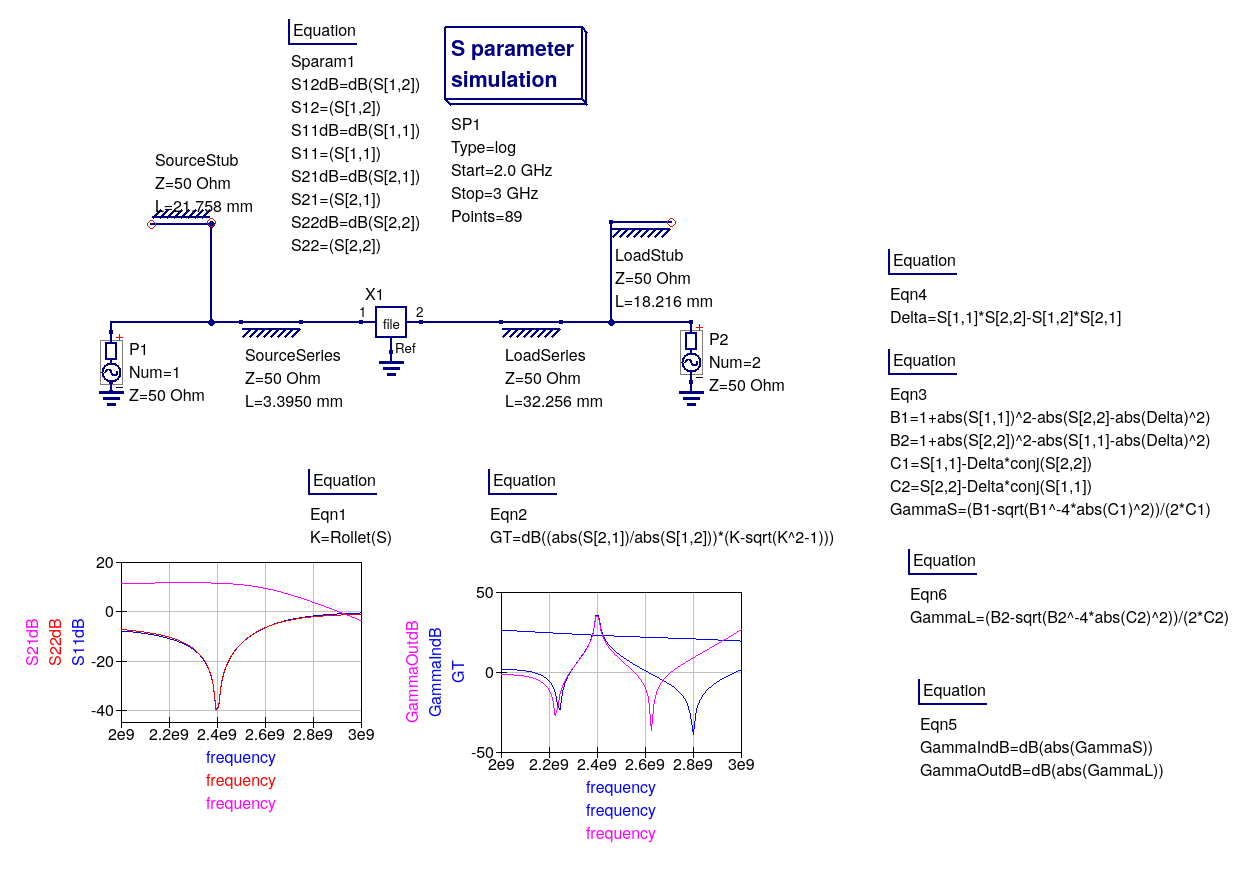
\includegraphics[width=100mm, scale=0.5]{Amp2_4GHzTLine.png}
  \caption{Amplifier with T-lines optimized for 2.4GHz}
  \label{fig4}
\end{figure}
We see the resonance of $\Gamma_{in}$ and $\Gamma_{out}$ which gives the
fact that a passive network can have gains larger than one.
The matching networks are in fact LC-tanks in resonance.
For 2.4GHz we have return loss taking the \v+dB+ of $S11$
of $2\times 44.6=89.2$dB.
\begin{figure}[H]
\centering
  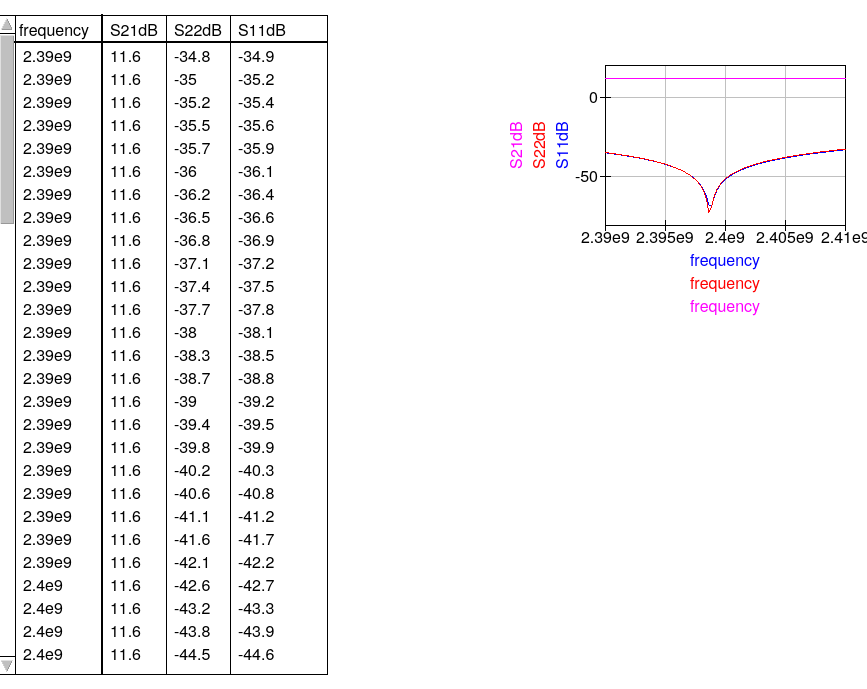
\includegraphics[width=80mm,scale=0.5]{Amp2_4GHzTLineData1.png}
  \caption{$G_T$ and returnloss for 2.4GHz}
  \label{fig4}
\end{figure}
For the specification of 2.45GHz it is somewhat lesser good because we had no
S-Parameters for this frequency I did not know how to extrapolate the figures
to 2.45GHz.
\begin{figure}[H]
\centering
  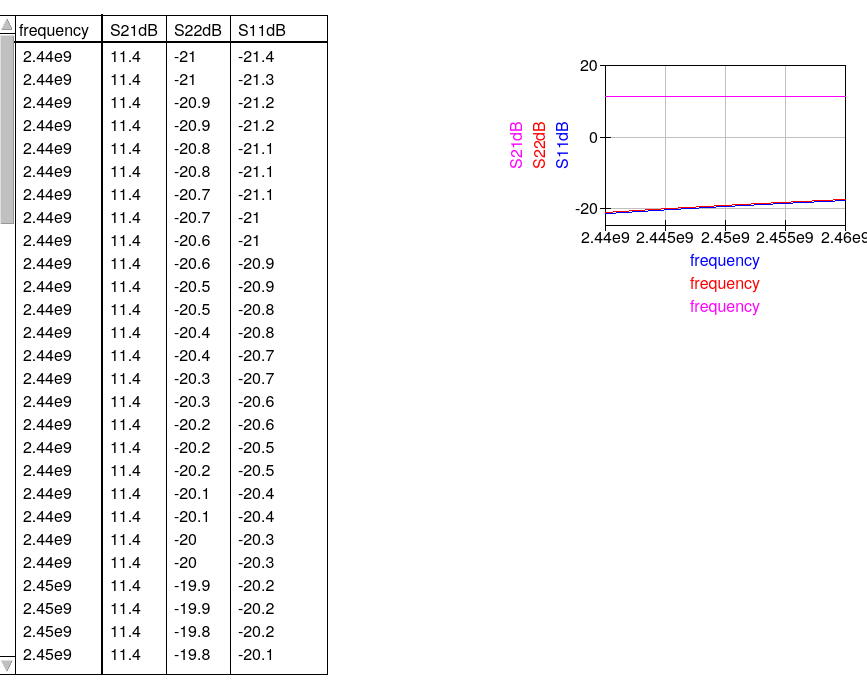
\includegraphics[width=80mm,scale=0.5]{Amp2_4GHzTLineData2.png}
  \caption{$G_T$ and returnloss for 2.45GHz}
  \label{fig4}
\end{figure}
We have returnloss of 40 dB and a tranceducer gain of 11.4 dB.
For the Microstrip version we calculated the effective
wavelength $\lambda_g$. We created the following code
to calculate $\epsilon_{eff}$ and the width of the microstrip
\begin{verbatim}
f=2.45E+9
c=3E+8
lambda= c/f;
ko=2*pi/lambda
epsilon_r=4.4
Z0=50
d=1.6E-3
loss_tangent=0.0018

%Accordin to Pozar's book
A=(Z0/60)*sqrt((epsilon_r +1)/2)+((epsilon_r-1)/(epsilon_r+1))*(0.23+0.11/epsilon_r)
B=(377*pi)/(2*Z0*sqrt(epsilon_r))

%For a given impedance Z0 and dielectric constant epsilon_r
%W/d-ratio calculated using the two formulas
%and the value is selected depinding if the output corresponds to the right restrictions
%on its origin
W2d_ratio1 =(8*exp(A))/(exp(2*A)-2)
W2d_ratio2 =(2/pi)*(B-1-log(2*B-1)+((epsilon_r-1)/(2*epsilon_r))*(log(B-1)+0.39-(0.61/epsilon_r)))
if(W2d_ratio1 <2)
 W2d_ratio = W2d_ratio1
 disp("Returned the first ratio")
elseif(W2d_ratio2 >2)
 W2d_ratio = W2d_ratio1
 disp("Returned the second ratio")
end
%Need epsilon effective for reduced wavelength
epsilon_eff = ((epsilon_r+1)/2)+((epsilon_r-1)/2)*(1/(sqrt(1+12*1/( W2d_ratio))))
attenuation_dielectric =(ko*epsilon_r*(epsilon_eff-1)*loss_tangent)/(2*sqrt(epsilon_eff)*(epsilon_r-1))

Width =  W2d_ratio*d
\end{verbatim}
The output is
\begin{verbatim}
f = 2.4500e+09
c = 3.0000e+08
ko = 51.313
epsilon_r = 4.4000
Z0 = 50
d = 1.6000e-03
loss_tangent = 1.8000e-03
A = 1.5299
B = 5.6463
W2d_ratio1 = 1.9119
W2d_ratio2 = 1.9134
W2d_ratio = 1.9119
Returned the first ratio
epsilon_eff = 3.3302
attenuation_dielectric = 0.076313
Width = 3.0590e-03
\end{verbatim}
Noticing now that I am cheating because the optimization is done for 2.4 GHz and
the idea was to just own the result of what the simulation gave us at 2.45GHz.
It was an error to use the wavelength corresponding to 2.45GHz!
\begin{figure}[H]
\centering
  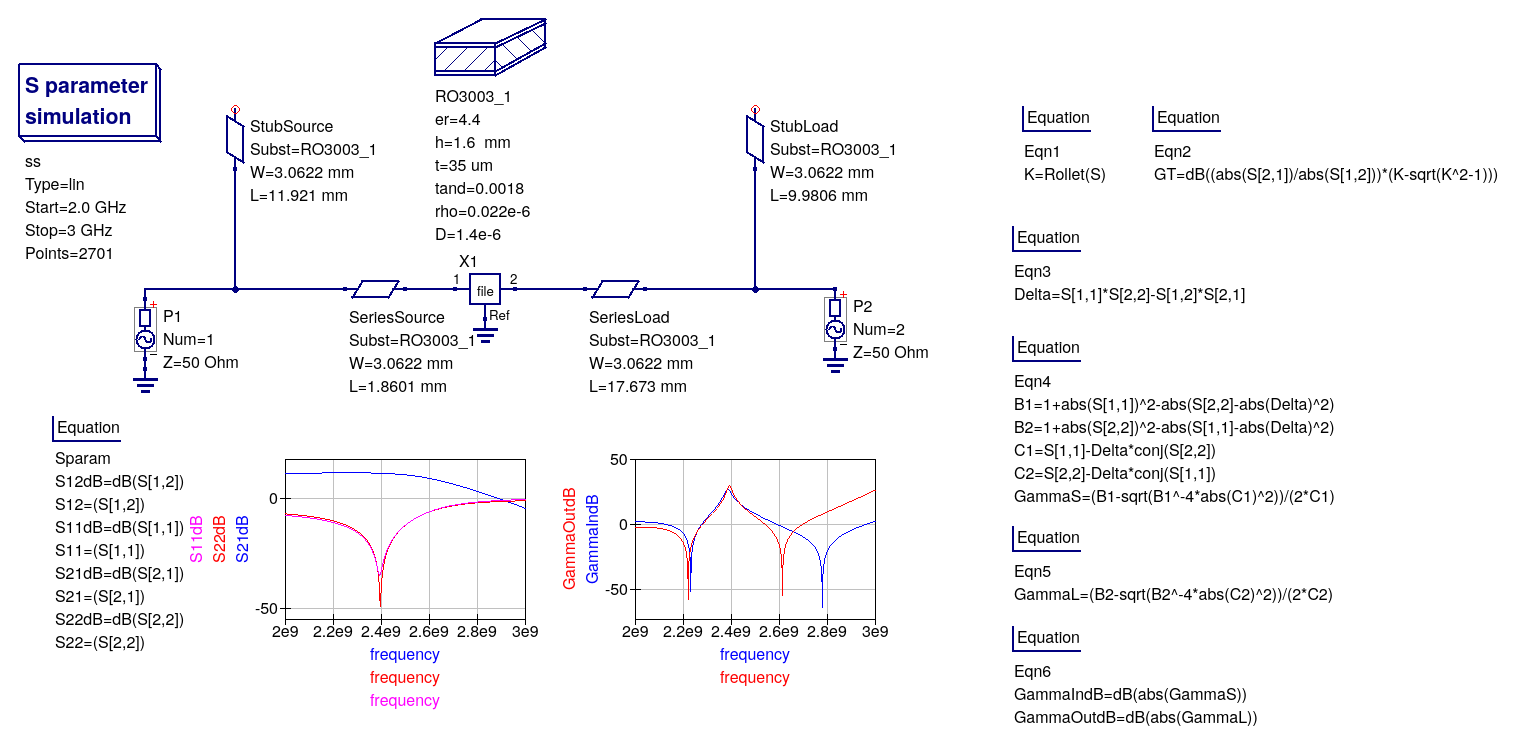
\includegraphics[width=80mm,scale=0.5]{Amp2_4GHzMicrostripNoTee.png}
  \caption{Amplifier with microstrip lines optimized for 2.4GHz}
  \label{fig4}
\end{figure}

Without Tee-bends

\begin{figure}[H]
\centering
  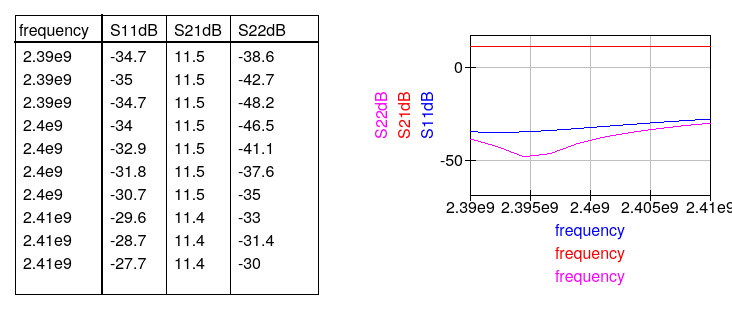
\includegraphics[width=80mm,scale=0.7]{Amp2_4GHzMicrostripNoTeeData1.png}
  \caption{$G_T$ and returnloss for 2.4GHz}
  \label{fig4}
\end{figure}
At 2.45 GHz we have $G_T = 11.2$dB and a returnloss of around 36dB.
\begin{figure}[H]
\centering
  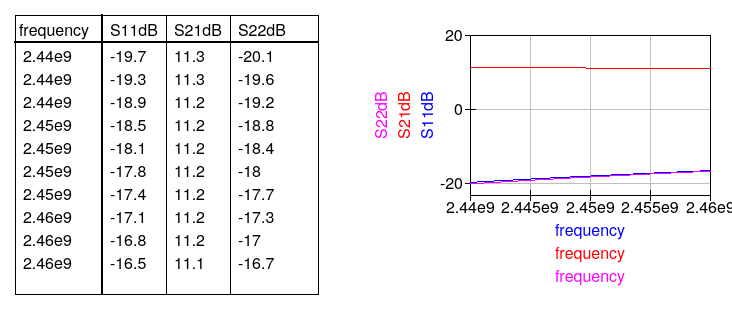
\includegraphics[width=80mm,scale=0.5]{Amp2_4GHzMicrostripNoTeeData2.png}
  \caption{$G_T$ and returnloss for 2.45GHz}
  \label{fig4}
\end{figure}
There is not much loss including the Tees.
Returnloss is 21 dB and and $G_T = 10.6$dB
\begin{figure}[H]
\centering
  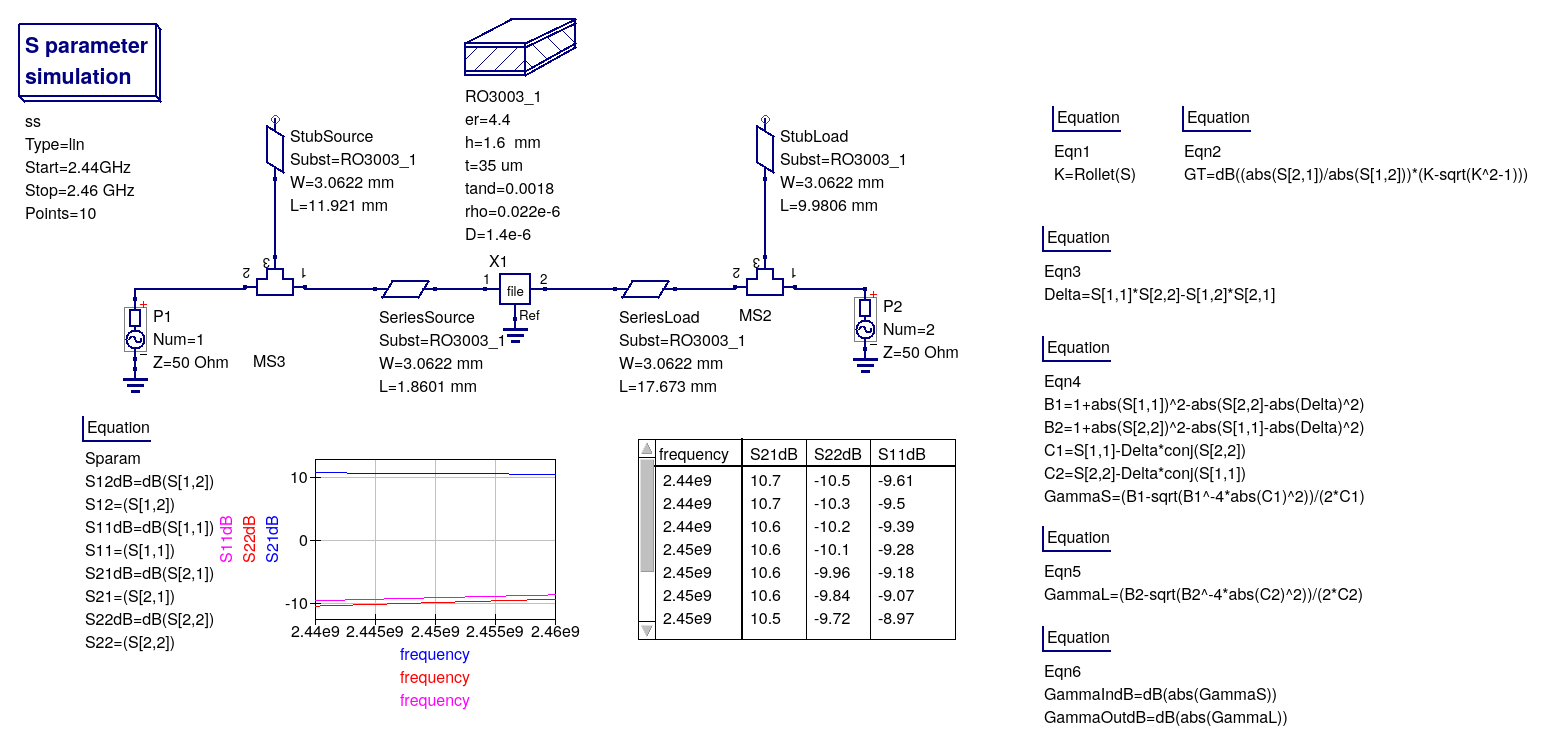
\includegraphics[width=\linewidth]{Amp2_4GHzMicrostripTee2.png}
  \caption{Amplifier with Tee-sections at 2.45GHz}
  \label{fig4}
\end{figure}

\section{Design for specific gain 13 dB (lowest possible Noise Figure)}
We wanted to design for an exact gain of 13 dB at 1.8 MHz with as small Noise-figure as possible.
We did not have noise-figure data for 1.8GHz so we used the data for 2.0 GHz.
We didn't follow the outline as presented by Pozar who describes the unilateral procedure
but followed the path described in
``Electromagnetic Waves \& Antenna''\footnote{\url{http://eceweb1.rutgers.edu/~orfanidi/ewa/}}
by Orfanidis using Availibel power -gain circles where
the load-side is matched which is also the preferred method
for desingning Low Noise Amplifiers.
We follwed the path outlined in the book and used his rudimentary matlab-toolbox ``ewa''
which is nevertheless much better than the complex RF-toolbox which is sold by Mathworks
though little editing had to be used because of older matlab-syntax and a
few plot-commands were in the somewhat wrong order and didn't display well.
 The minimum Noise Figure was found to be 1.96 dB at 13dB of gain
where we didn't account for microstrip losses.


\begin{multicols}{2}
Plotting the components of the trancducer gain we noticed that the output matching network was damping
\begin{verbatim}
Gains of matching networks
G_S = 2.2933
G_S_dB = 3.6047
G_L = 0.8760
G_L_dB = -0.5749
Gt gain
Total_Gain = 27.831
Total_Gain_dB = 14.445
\end{verbatim}
We didn't want to add more damping
so we diecided for the availible power gain approach
The Noise-figure for a conjugate match
The optimal refelction coefficient for the noise figure
taken from the touchstone-file was used and the corresponding
$\Gamma_{out}$ calculated with the standard formula
\begin{flalign*}
\Gamma_{out} &= S_{22}+\frac{S_{12}S_{21}\Gamma_S}{1-S_{11}\Gamma_S}
\end{flalign*}
The availible gain at optimal nois-figure was recorded
and the corresponding $\Gamma_L=\Gamma_{out}^*$
noted
\begin{verbatim}
disp("Noise figure calculations")
%From Touchstone file at 2 000 MHz
%2000  1.90  .242  134.0   .160
Fmin = 1.90;  rn = 0.16;
%Optimal NF GammaS reflection coeff
gGopt = p2c(0.242 ,134.0 );
% maximum available gain
Gmag = db(sgain(S,'mag'))
% available gain at GammaS opt
Gaopt = db(sgain(S,gGopt,'a'))
% matched load
gLopt = conj(gout(S,gGopt))  
figure;
smith;
plot(gGopt,'*r')
plot(gLopt,'xk')
\end{verbatim}
The output
\begin{verbatim}
Noise figure calculations
Gmag = 14.445
Gaopt = 12.304
gLopt =  0.1528 + 0.3450i
\end{verbatim}
We see that the reflection coefficient giving
the optimal noisefigure of 1.9 dB does not give
an availible Gain $G_A$ of 13 dB which is our target.
Hence we must allow for a higer noise figure.
We plot on the Smith chart the the optimal noise reflection coefficient for the source
and its corresponding conjugate to $\Gamma_{out}$ which means
that the output is conjugately matched  
\begin{figure}[H]
\centering
  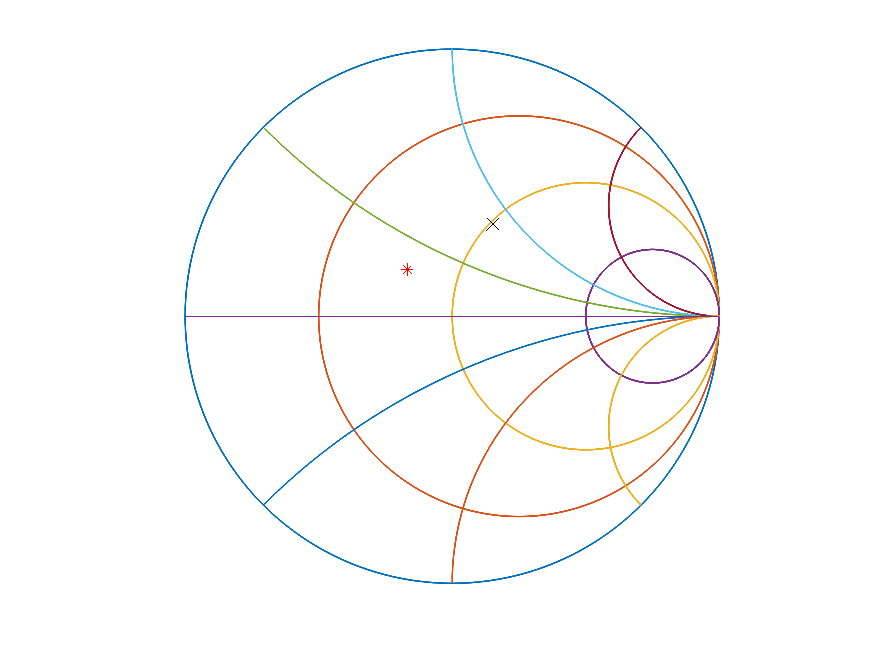
\includegraphics[width=\linewidth]{optimal_noisefigureGamma.png}
  \caption{$\Gamma_{S,optN}$ (*) and $\Gamma_L=\Gamma_{out}^*$(x)}
  \label{fig4}
\end{figure}
We plot Noise figure cirlces for 1.95, 1.96,2.1 and 2.2 dB on the chart
\begin{verbatim}
[c0,r0]=nfcirc(1.9,Fmin,rn,gGopt);
[c1,r1]=nfcirc(1.95,Fmin,rn,gGopt);
[c2,r2]=nfcirc(1.96,Fmin,rn,gGopt);
[c3,r3]=nfcirc(2.1,Fmin,rn,gGopt);
[c4,r4]=nfcirc(2.2,Fmin,rn,gGopt);

smithcir(c0,r0);%A point only
plot(c0,'*')%Same point as previously
smithcir(c1,r1);
plot(c1,'*')
smithcir(c2,r2);
plot(c2,'*')
smithcir(c3,r3);
plot(c3,'*')
smithcir(c4,r4);
plot(c4,'*')
\end{verbatim}
We notice that the circles have almost the same
center-point and the fact that these are circles
stem for the fact that there are many reflection coefficients
that can accomplish a certain Noise figure greater than the minimal NF.
\begin{figure}[H]
\centering
  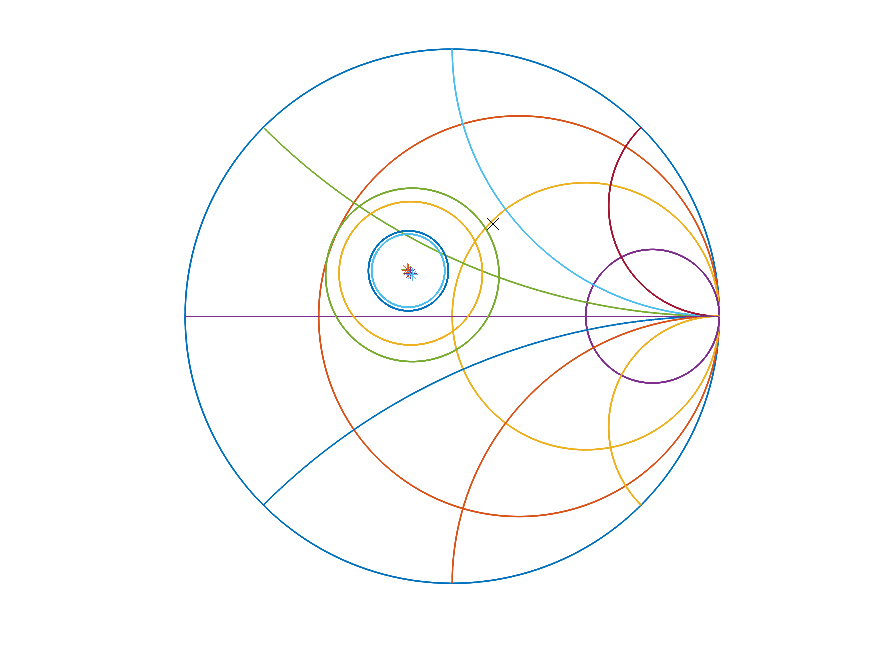
\includegraphics[width=\linewidth]{NoisefigureCircles.png}
  \caption{Constant Noise-figure circles at 1.95,1.96, 2.0 and 2.2 dB}
  \label{fig4}
\end{figure}
What is the noise figure for the conjugate match?
We calculate it and we also plot the optimal reflection
coefficients for the conjugate match which gives 14.445 dB gain.
\begin{verbatim}
[gG,gL] = smatch(S)
plot([gG,gL],'*g')
F = nfig(Fmin, rn, gGopt, gG)
\end{verbatim}
Output is
\begin{verbatim}
gG = -0.7395 - 0.1306i
gL =  0.4402 + 0.5100i
F = 3.8037
\end{verbatim}
The noise figure for the max gain case (14.445 dB) is 3.8037 dB.
\begin{figure}[H]
\centering
  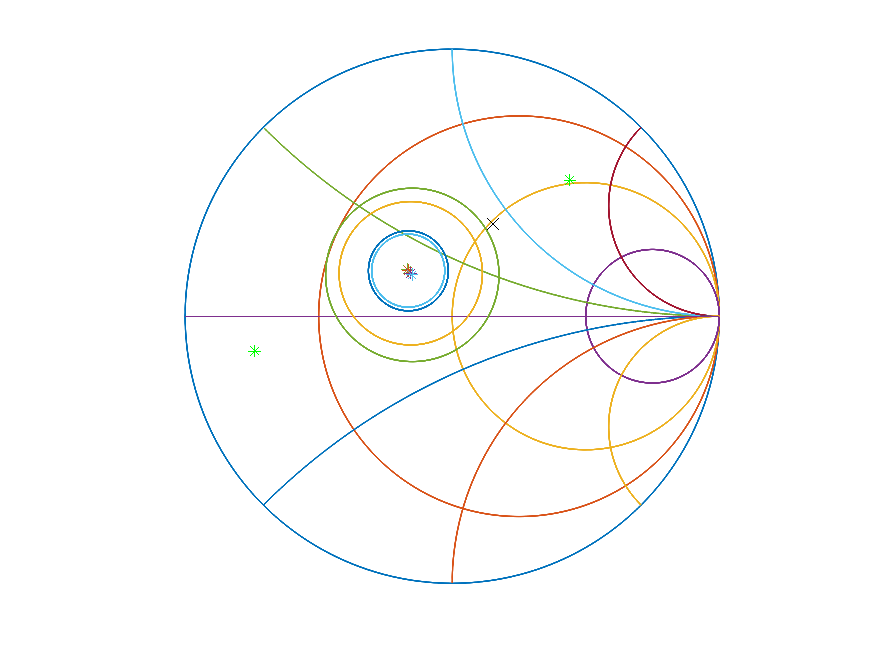
\includegraphics[width=\linewidth]{conjugate.png}
  \caption{Green stars added for max gain cojugate match reflection coefficients. $\Gamma_S$ is down left}
  \label{fig4}
\end{figure}
Next we want to store all source reflection coefficients related to a particular
Noise figure circle we are interested in and calculate the gain for
each of these circles and pick out the one which gives an availibel power gain
of 13 dB.
We either know from first hand which noise-figure circle
or we tested to see which gains were associated
\begin{verbatim}
%Create an array of phi-values
%in incremenets of a half degree
%from 0 to 2$\pi$
phi = linspace(0,2*pi,721);
% Record the GammaG's around the c 2 , r 2 circle
gGammas = c2 + r2*exp(j*phi);
% Calculate the available gain in dB
G = db(sgain(S,gGammas,'a'));
%Pick out the index with the
%highest gain
[Ga,i] = max(G) 
%If you need to search for a gain on
%the circle use this code
find an index in array of a specific gain
index=1;
sizeG = 721;
for(i=1:1:sizeG)
%G(i)
%Edit the gain values for a different gain
 if (G(i)>13.0 ) && (G(i)<13.1)
   index=i
   G(i)
   disp("found index")
   break;
 endif
end
% GammaS for maximum gain
%if you already know the correct
%Noise-figure circle and just
%want to pick the highest gain
%of corresponding noise-figure circle
gammaS = gGammas(i) 
%If you look for a specific gain
%run this line instead
%gammaS = gGammas(index) 
\end{verbatim}
Output is
\begin{verbatim}
Ga = 13.001
i = 427
sizeG = 721
gammaG = -0.289592 + 0.088463i
\end{verbatim}
so the maximum availible gain $G_A$ on the 1.96 dB Noise figure circle
happen to be 13.001 and the corresponding $\Gamma_S$ value
is -0.289592 + 0.088463i.

We want to calculate $\Gamma_{out}$ for this value of $\Gamma_S$
with the standard formula
and take the conjugate and assign that conjugate value to
$\Gamma_L$.
\begin{flalign*}
\Gamma_{out} &= S_{22}+ \frac{S_{21}S_{21}\Gamma_S}{1-S_{11}\Gamma_S}\\
           \Gamma_L &=\Gamma_{out}^*
\end{flalign*}
 We also want to plot the availibe gain circles
for 13 dB and see if it has common points with the 1.96 dB
Noise figure circle.
We also want to plot the the $\Gamma_S$ that we found and it should
lie on the 13 dB availible gain circle as well as on the 1.96 dB
Noise-figure circle.
\begin{verbatim}
gammaL = conj(gout(S,gammaG))
% Available gain circle 13.001 dB
[ca,ra] = sgcirc(S,'a',Ga);
%Center point with a red asterix
plot(ca,'*r')
smithcir(ca,ra);
%GammaG and GammaL added to Smitchart
%with blue asterix
plot([gammaS,gammaL],'*b');
\end{verbatim}

\begin{figure}[H]
\centering
  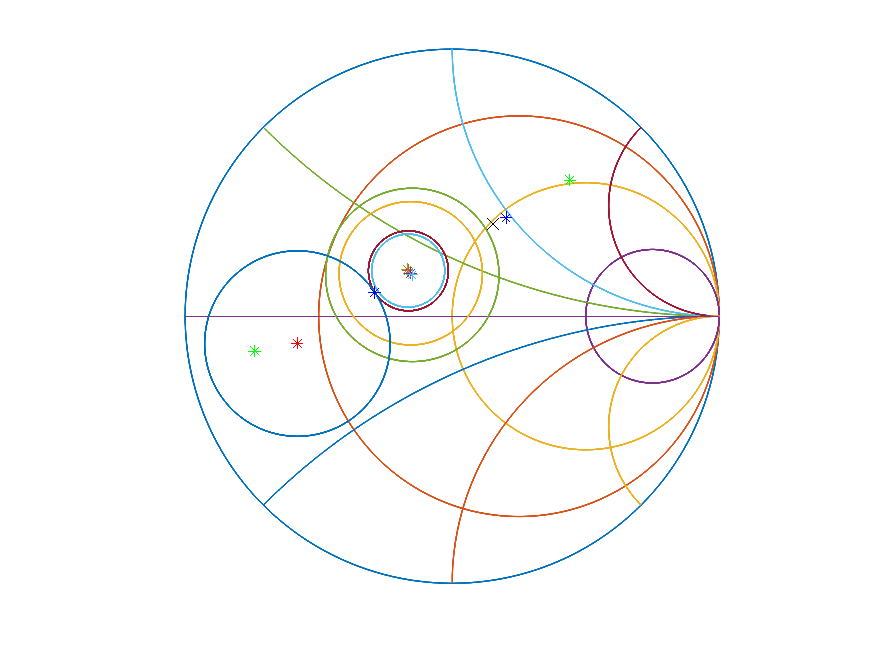
\includegraphics[width=\linewidth]{FinalNoiseFig.png}
  \caption{13 dB Availible gain circle with corresponding $\Gamma_S$ reflection coefficient added with blue asterix which rests on
 13 db availible gain circle and 1.96 dB Noise figure circle. Corresponing $\Gamma_L$ also added with a blue asterix}
  \label{fig4}
\end{figure}

We provide a plot to illustrate how
the availible power gain varies
on the 1.96 dB Noise-figure circle
and calculate the stub lengths
and the serial lines
\begin{verbatim}
figure
plot(phi*180/pi, G);
zG=(1+gammaG)/(1-gammaG)
zL=(1+gammaL)/(1-gammaL)
dl_IN_noiseFig = stub1 (conj(zG), 'po' )
dl_OUT_noiseFig = stub1 (conj(zL), 'po' )
lambda_mm=1000*3E8/1.8E9
stub_in_mm = dl_IN_noiseFig(2,1)*lambda_mm
serial_in_mm=dl_IN_noiseFig(2,2)*lambda_mm

stub_out_mm = dl_OUT_noiseFig(2,1)*lambda_mm
serial_out_mm=dl_OUT_noiseFig(2,2)*lambda_mm
\end{verbatim}

\begin{figure}[H]
\centering
  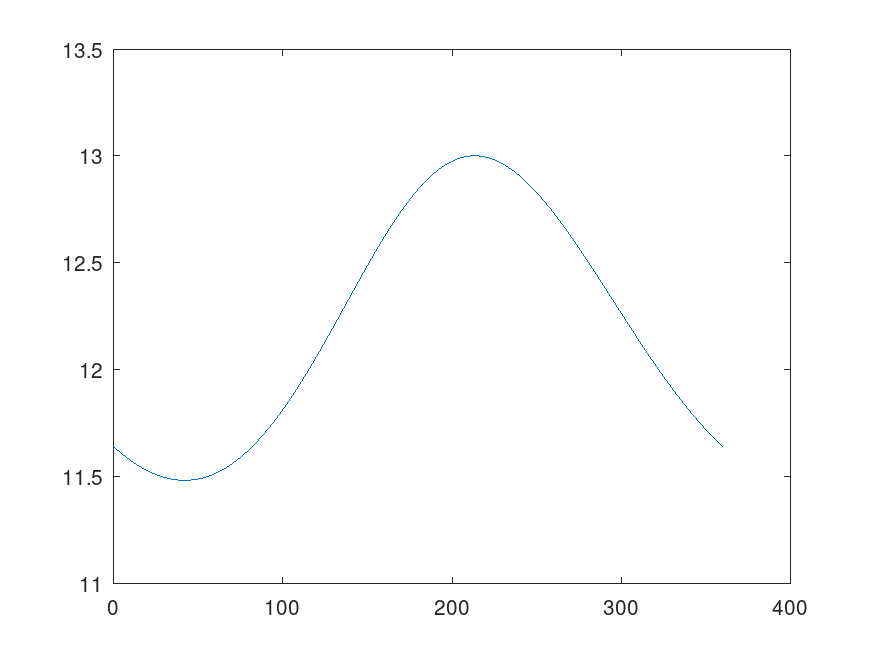
\includegraphics[width=\linewidth]{GainVariationOnNoisefigCircle.png}
  \caption{The variation of the availible gain with respect to the $Gamma_S$ reflection coefficients related to the 1.96 dB Noisefigure circle}
  \label{fig4}
\end{figure}
Remark: It is the conjugate of $Z_G$ and $Z_S$
which are the impedances looking into the DUT
which should be tranformed to 50 Ohms.
We are always walking "Towards the load" on the Smitchart
both for the load side and the source side.
The problem is identical to a beginner's load matching problem
except there one always traverses the Smitchart "towards the generator".
Output
\begin{verbatim}
lambda_mm = 166.67
stub_in_mm = 15.015
serial_in_mm = 20.685
stub_out_mm = 19.825
serial_out_mm = 42.568
\end{verbatim}
We've calculate
the width of the microstrip and how to calculate
$\epsilon_{eff}$ for the formula $\lambda_{eff}= \lambda/\sqrt{\epsilon_{eff}}$
\end{multicols}

%%
\begin{figure}[H]
\centering
  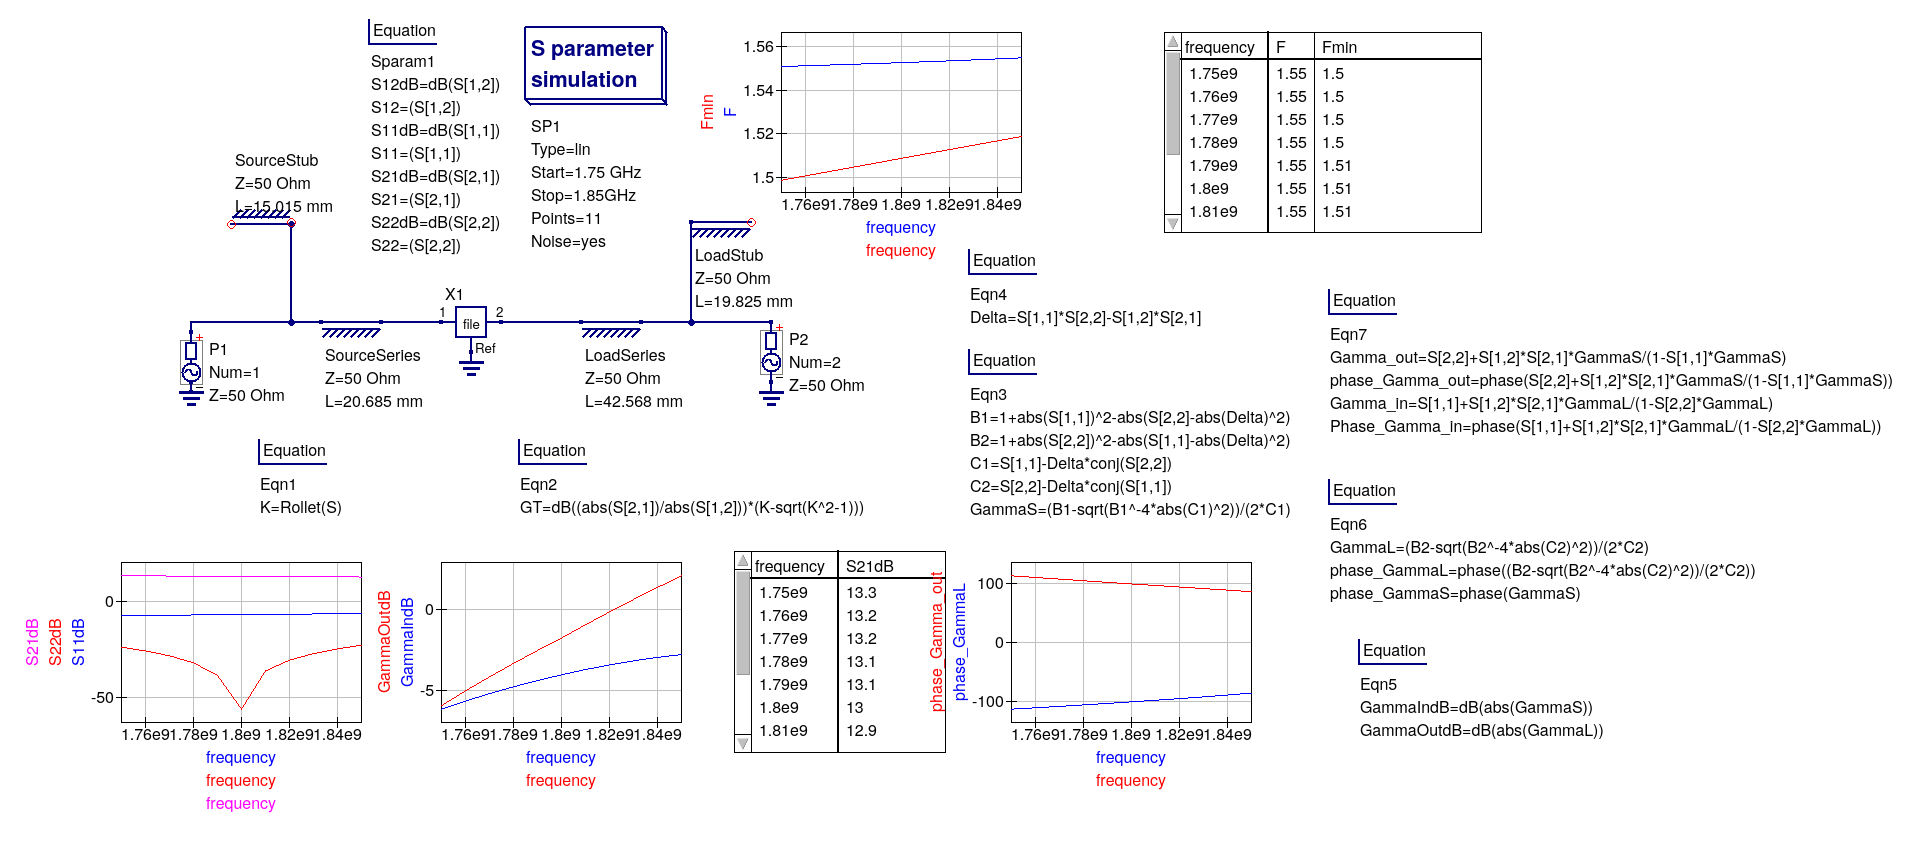
\includegraphics[width=\linewidth]{X1800MHzAt13dBAt2dBNF.png}
  \caption{Design with theoretical TLINE transmissionlines}
  \label{fig4}
\end{figure}
The formula for \verb+GammaIndB+ and \verb+GammaOutdB+ are not correct but had followed along from the
conjugated matched design. They are corrected in the longer sweep below.
The Noise-fige plot is not correct but should be higher. Minimum NF should be
1.9 dB at 2 GHz according to the Touchstone file
\begin{verbatim}
! Noise data:
! Freq.     Fmin        Gamma-opt         rn
  500       1.10     .330     27.0       .250
  900       1.25     .294     48.0       .260
 1000       1.30     .298     52.0       .270
 2000       1.90     .242    134.0       .160
\end{verbatim}
The program locks often so we couldn't rearrange the graphics as to not
overlap. Here we do a sweep from 1.5 to 3GHz

\begin{figure}[H]
\centering
  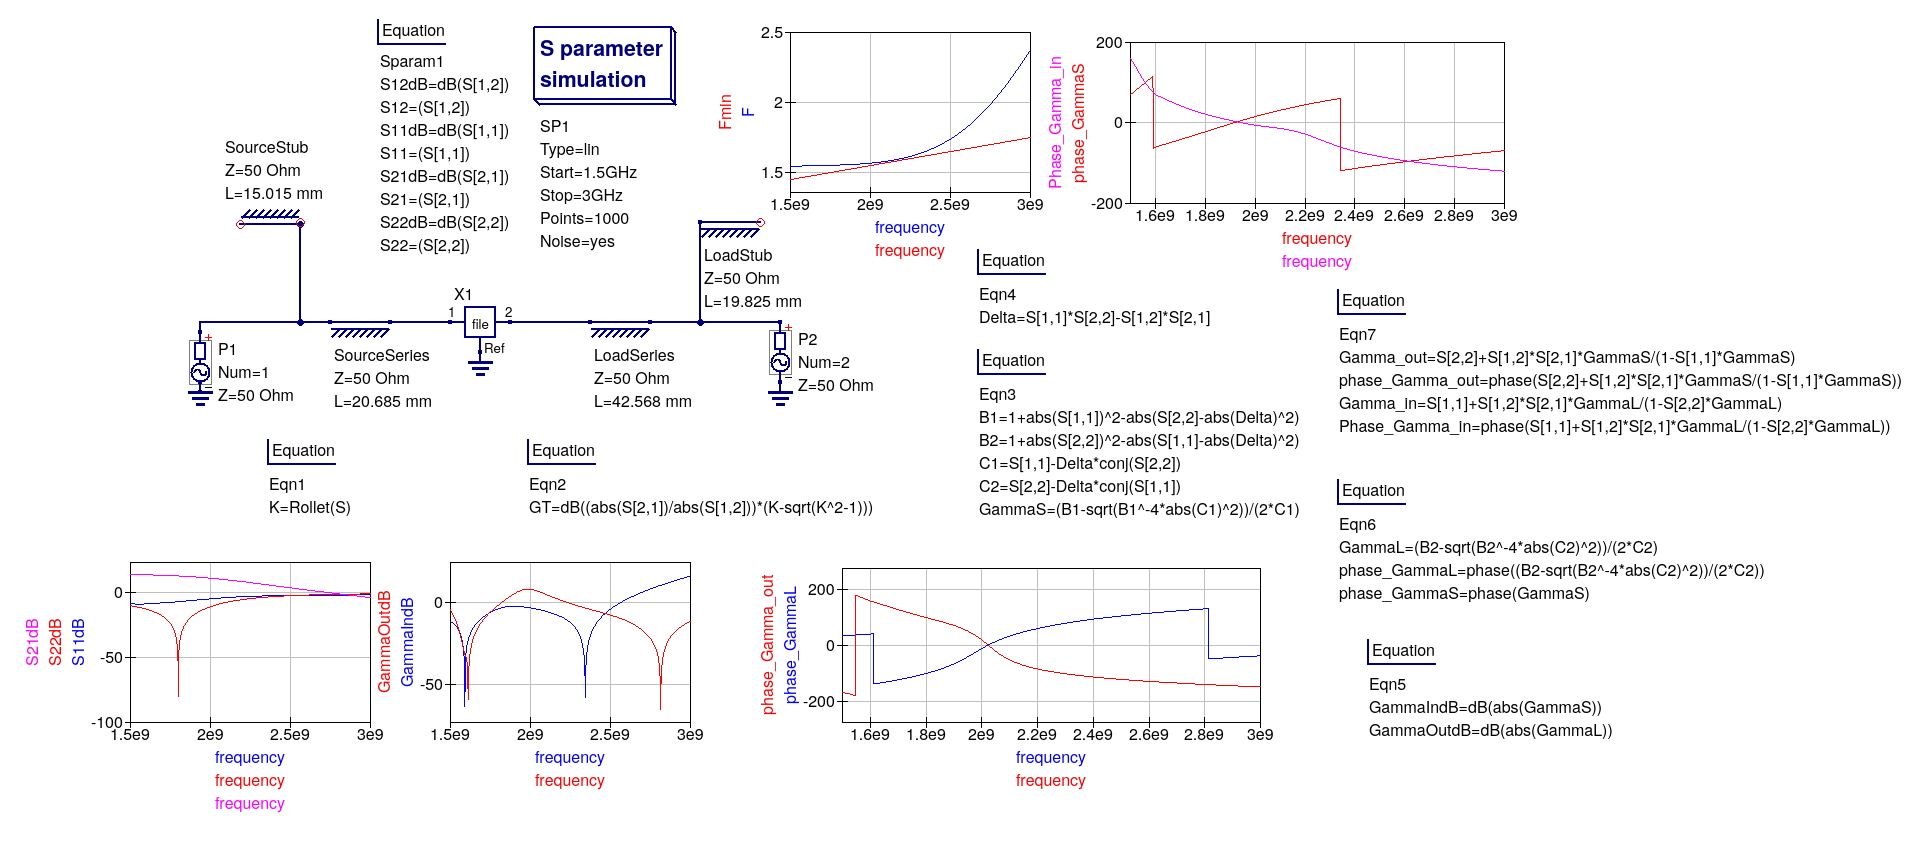
\includegraphics[width=\linewidth]{X21800MHzAt13dBAt2dBNF.png}
  \caption{Design with theoretical TLINE transmissionlines. Longer sweep}
  \label{fig4}
\end{figure}

Calculation of microstrip lengths

\begin{verbatim}
disp("Microstrips")
d=1.6E-3;
epsilon_r = 4.4;
losstangent = 0.0018
copper_thickness = 34E-6;
u=mstripr(epsilon_r,50);
e_eff= mstripa(epsilon_r,u);
lambda_eff_mm =lambda_mm/sqrt(e_eff)
Width = u*d

stub_in_mm = dl_IN_noiseFig(2,1)*lambda_eff_mm
serial_in_mm=dl_IN_noiseFig(2,2)*lambda_eff_mm

stub_out_mm = dl_OUT_noiseFig(2,1)*lambda_eff_mm
serial_out_mm=dl_OUT_noiseFig(2,2)*lambda_eff_mm
\end{verbatim}
Noticing the difference in the wave length!
\begin{verbatim}
lambda_eff_mm = 91.315
Width = 3.0622e-03
stub_in_mm = 8.2268
serial_in_mm = 11.333
stub_out_mm = 10.862
serial_out_mm = 23.322
\end{verbatim}
The Noise figure calculation is still rubbish but we have still have 13 dB gain
\begin{figure}[H]
\centering
  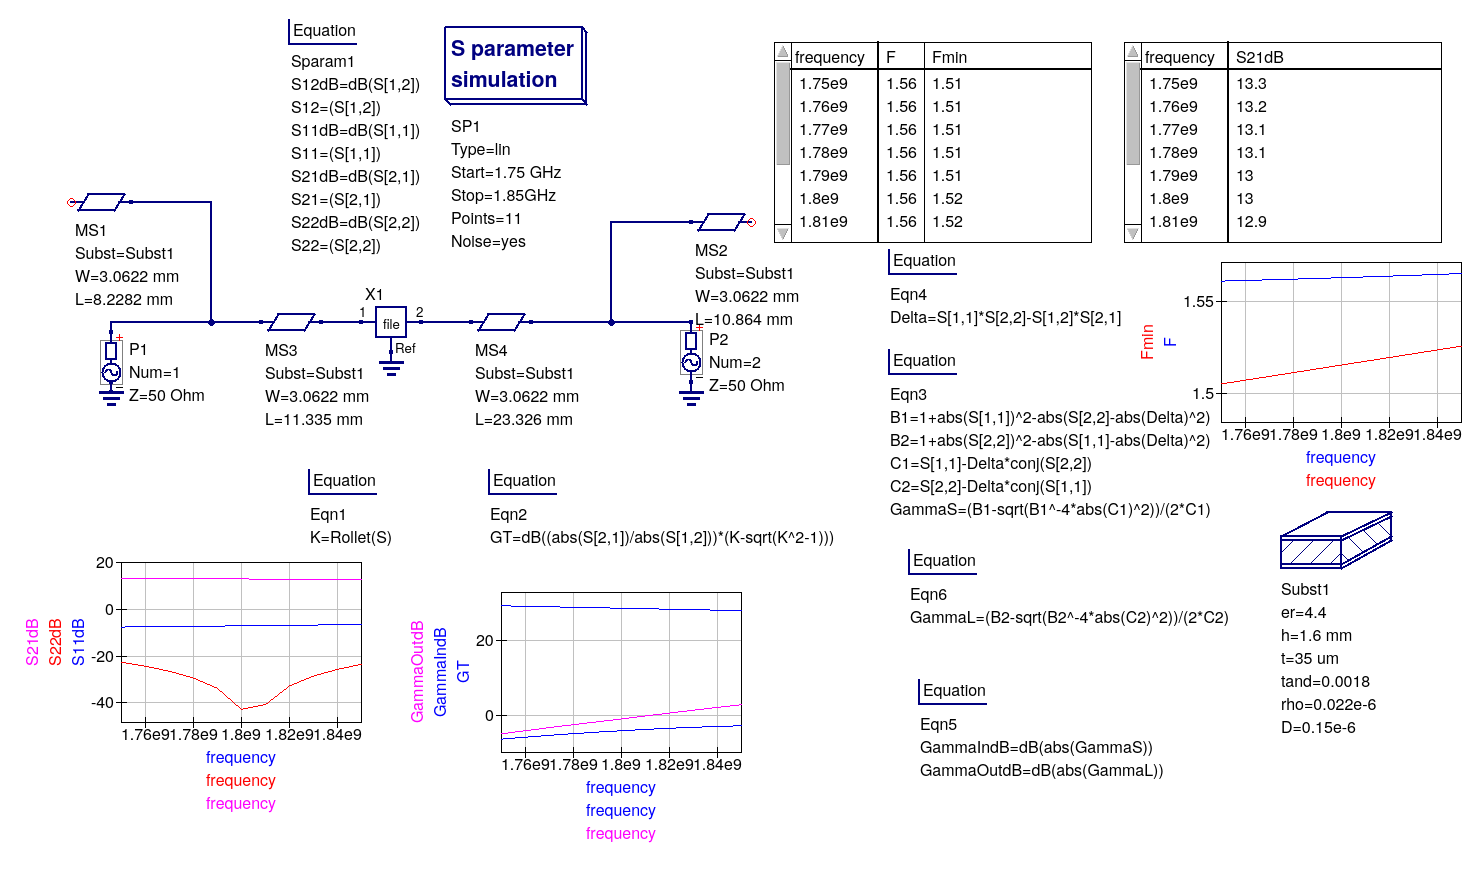
\includegraphics[width=\linewidth]{1800MHzAt13dBAt2dBNF.png}
  \caption{Design with microstrip lines}
  \label{fig4}
\end{figure}
A longer sweep. Something unphysical happens with $\Gamma_{in}$ at 2.1 GHz which
is not reflected upon the composite $S_{11}$.


\begin{figure}[H]
\centering
  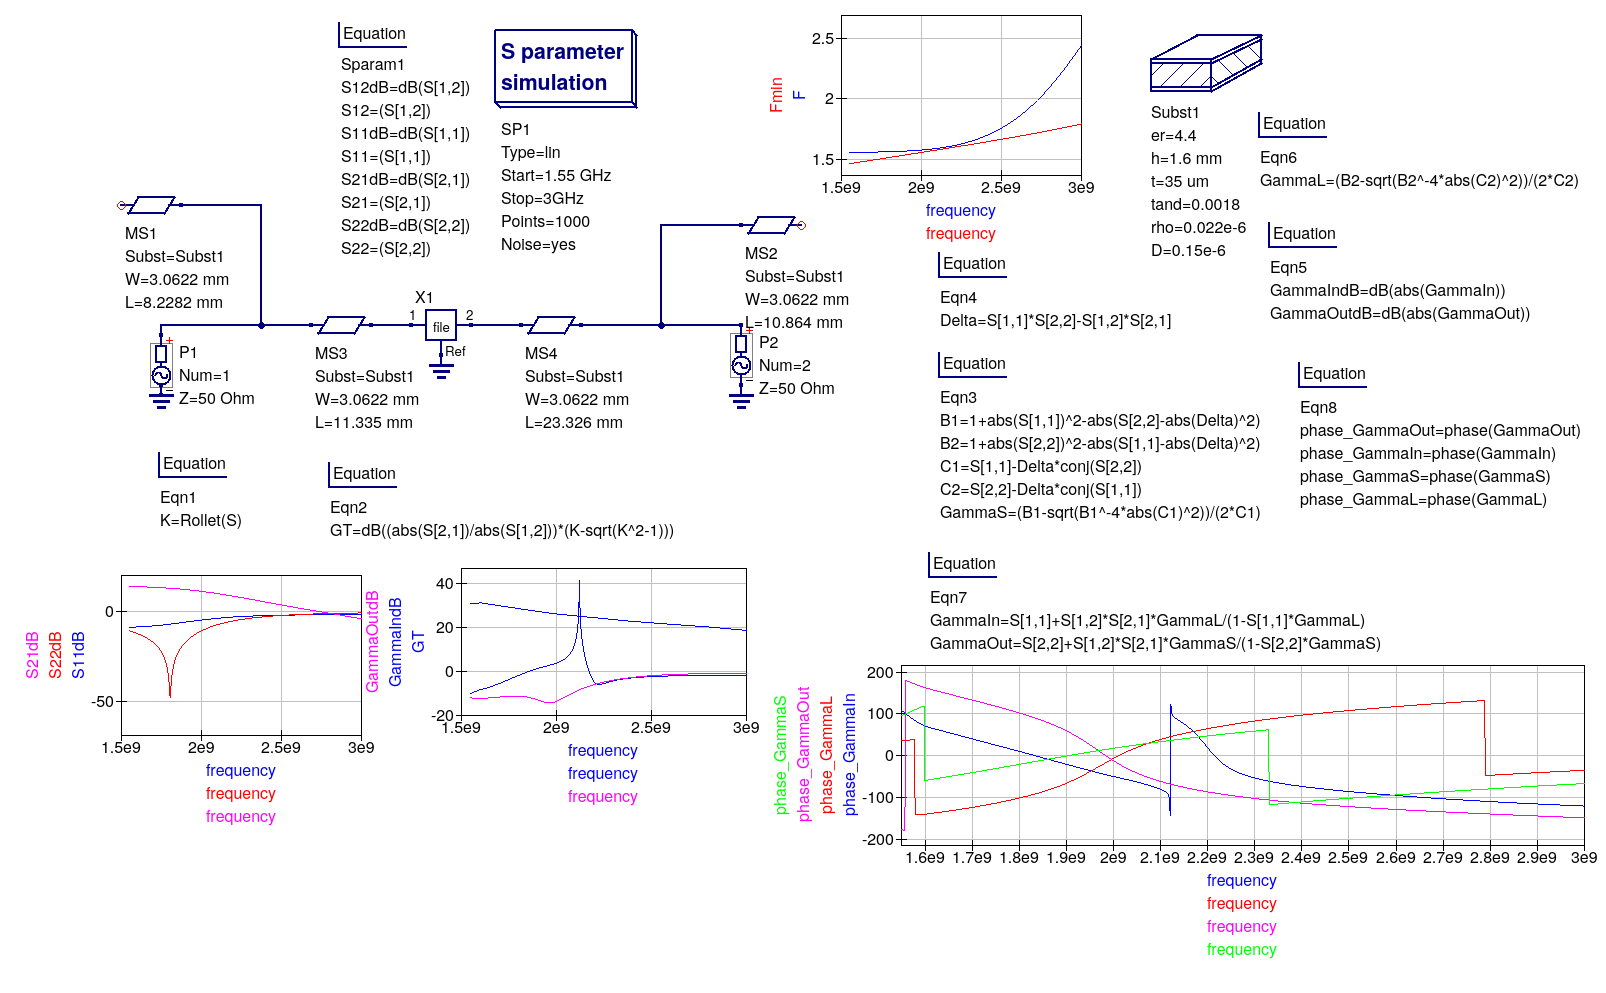
\includegraphics[width=\linewidth]{X1800MHzAt13dBAt2dBNFSweep.png}
  \caption{Design with microstrip lines. Longer sweep}
  \label{fig4}
\end{figure}
Not much losses including Tee-bends

\begin{figure}[H]
\centering
  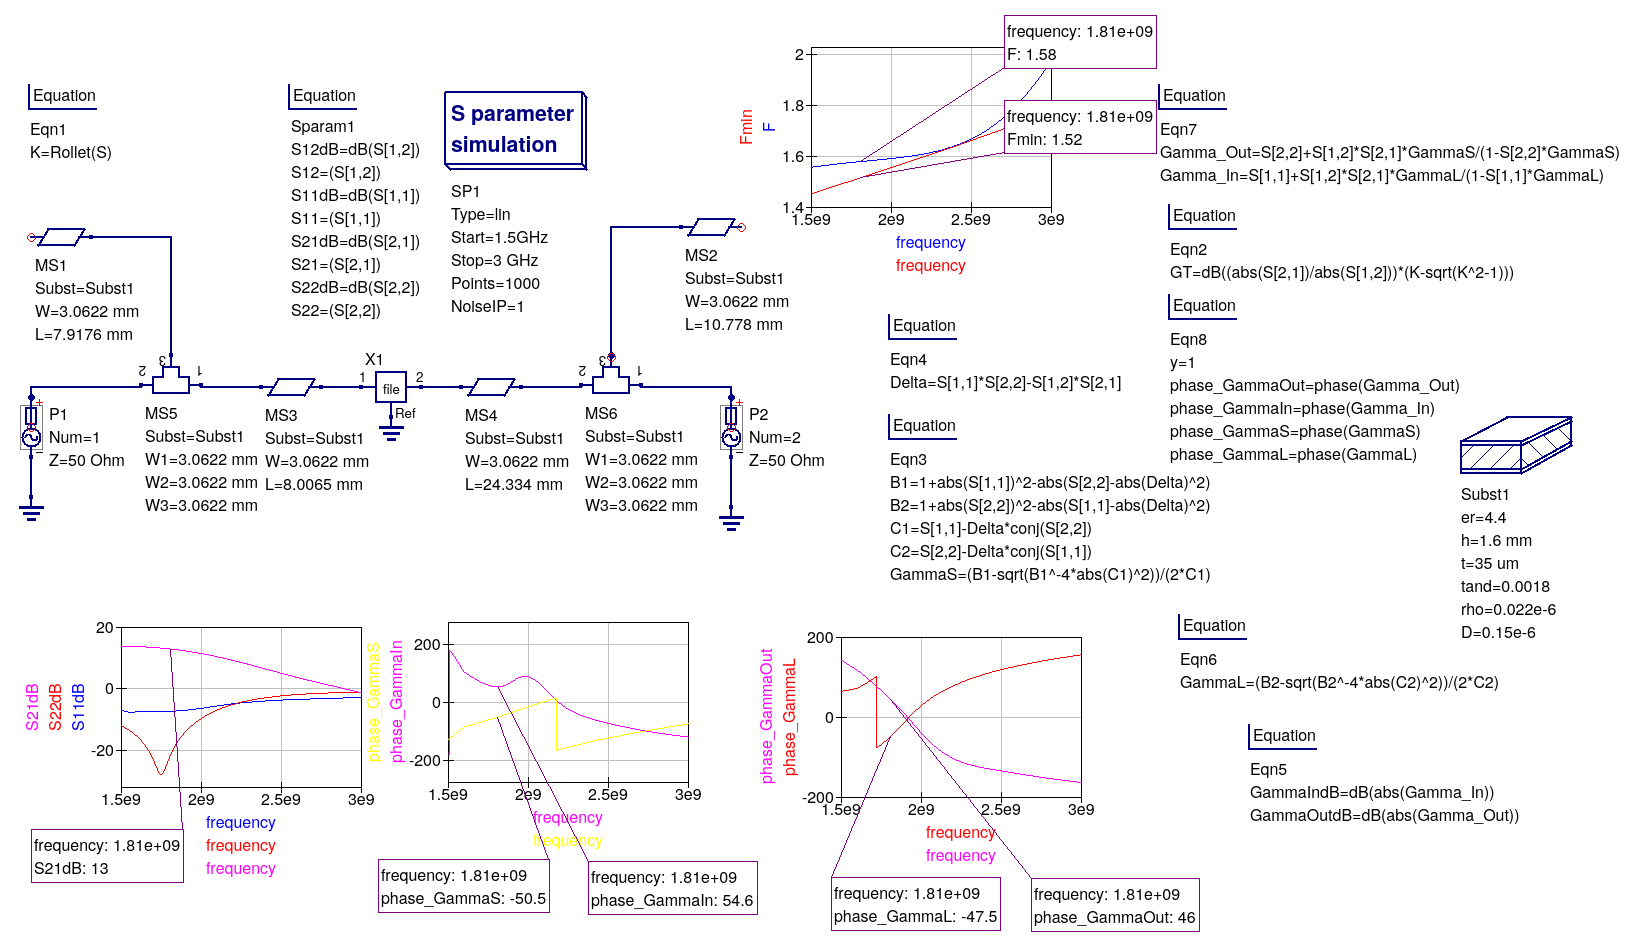
\includegraphics[width=\linewidth]{TEE1800MHzAt13dBAt2dBNFSweep.png}
  \caption{Design with microstrip Tees}
  \label{fig4}
\end{figure}

What about if we simulate for integer values of the microstrips lengths?
\begin{figure}[H]
\centering
  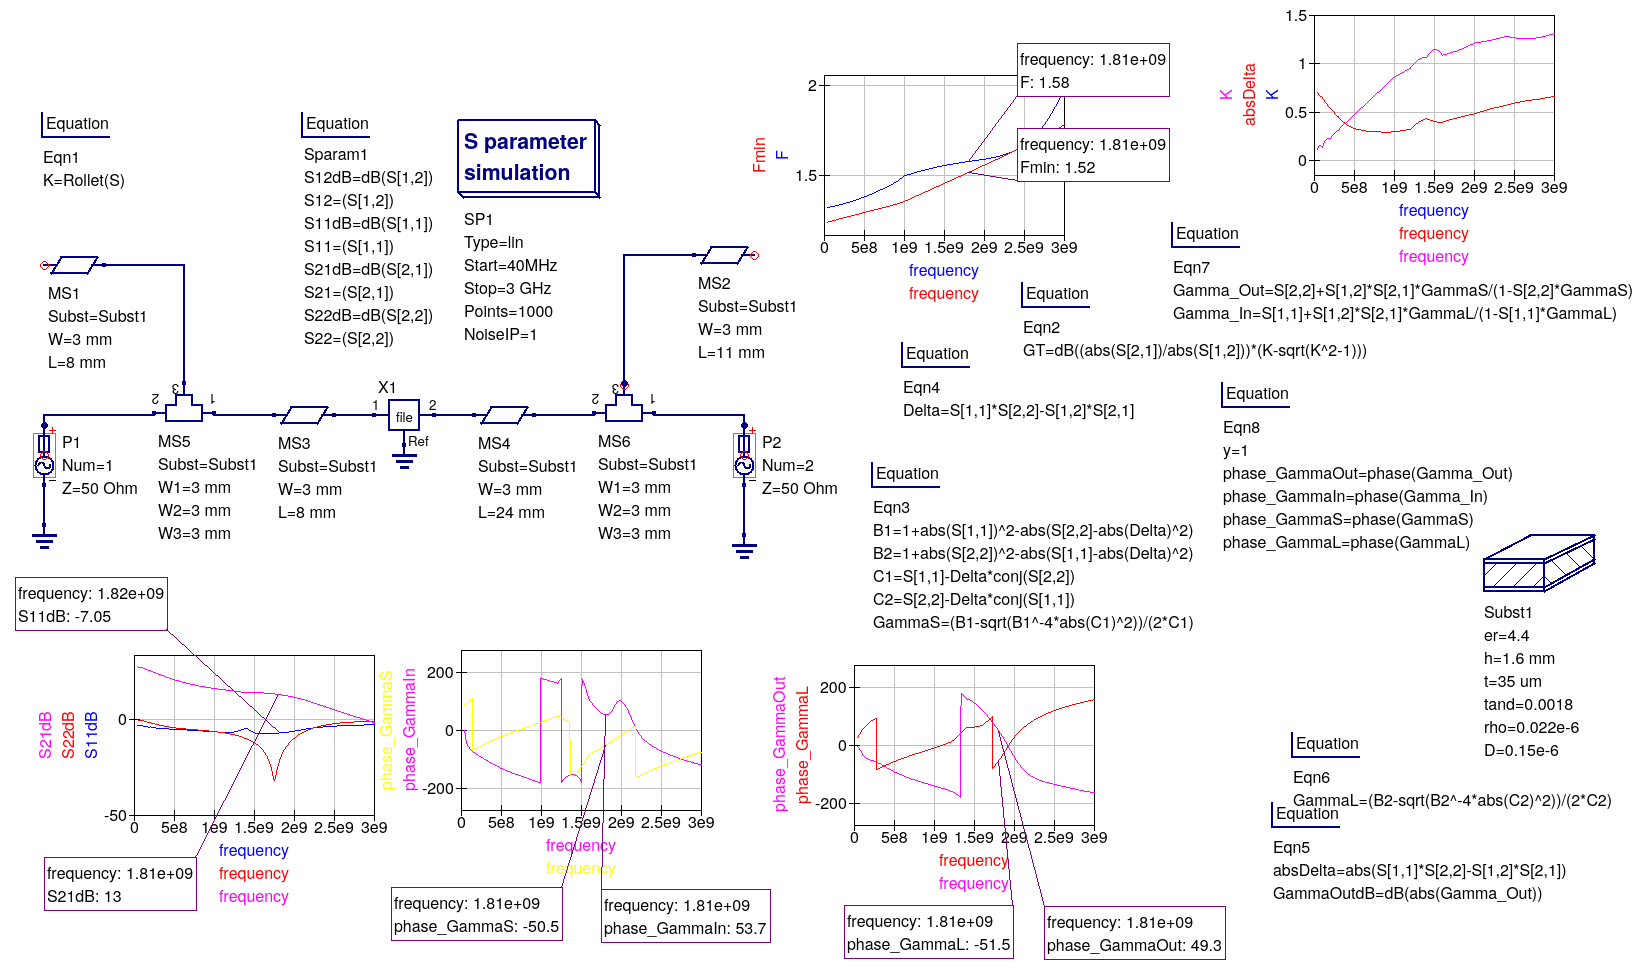
\includegraphics[width=\linewidth]{TEE1800MHzAt13dBAt2dBNFSweep2.png}
  \caption{Design with microstrip Tees}
  \label{fig4}
\end{figure}
Still not stable over all frequencies because we have still not done
any stabilization. Still have the correct gain. Returnloss is around 14 dB at

\section{Implementation for specific gain 13 dB (lowest possible Noise Figure)}

We choose the implementation without Tees which is the following circuit
referenced previously
\begin{figure}[H]
\centering
  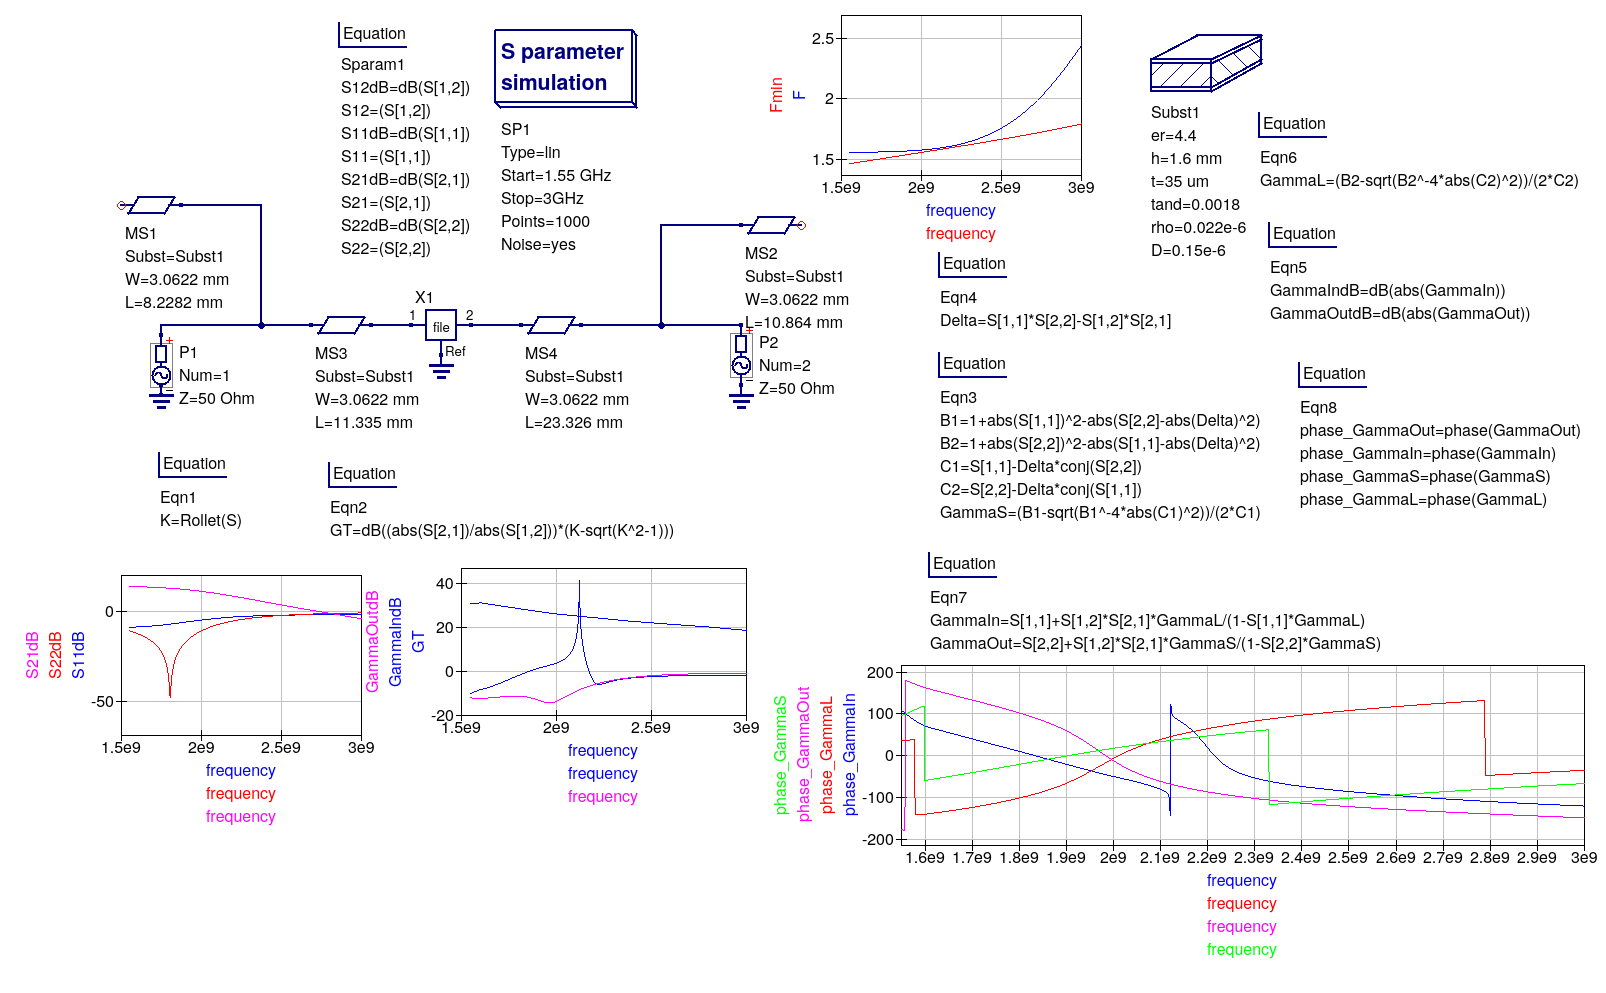
\includegraphics[width=\linewidth]{X1800MHzAt13dBAt2dBNFSweep.png}
  \caption{Design with microstrip lines. Longer sweep}
  \label{fig4}
\end{figure}

It was implemented using copper tape on an FR4-board and bias tees of type ZFBT-6G
from Minicircuits\footnote{\url{https://www.minicircuits.com/WebStore/dashboard.html?model=ZFBT-6G\%2B}} were used on the 
input as well as o the output. These circuts have an insertion loss of ca 0.4 dB and an VSWR of ca 1.12
at 1800 MHz\footnote{\url{https://www.minicircuits.com/pages/s-params/ZFBT-6G+_GRAPHS.pdf}}

\begin{figure}[H]
\centering
  \includegraphics[width=\linewidth]{photos/circuit.png}
  \caption{Circuit with copper tape as microstrip lines}
  \label{fig4}
\end{figure}

The VNA used to measure $S_{11}$ and  $S_{21}$ was the NanoVNA, type SAA2\footnote{\url{https://nanorfe.com/nanovna-v2.html}}.
\begin{figure}[H]
\centering
  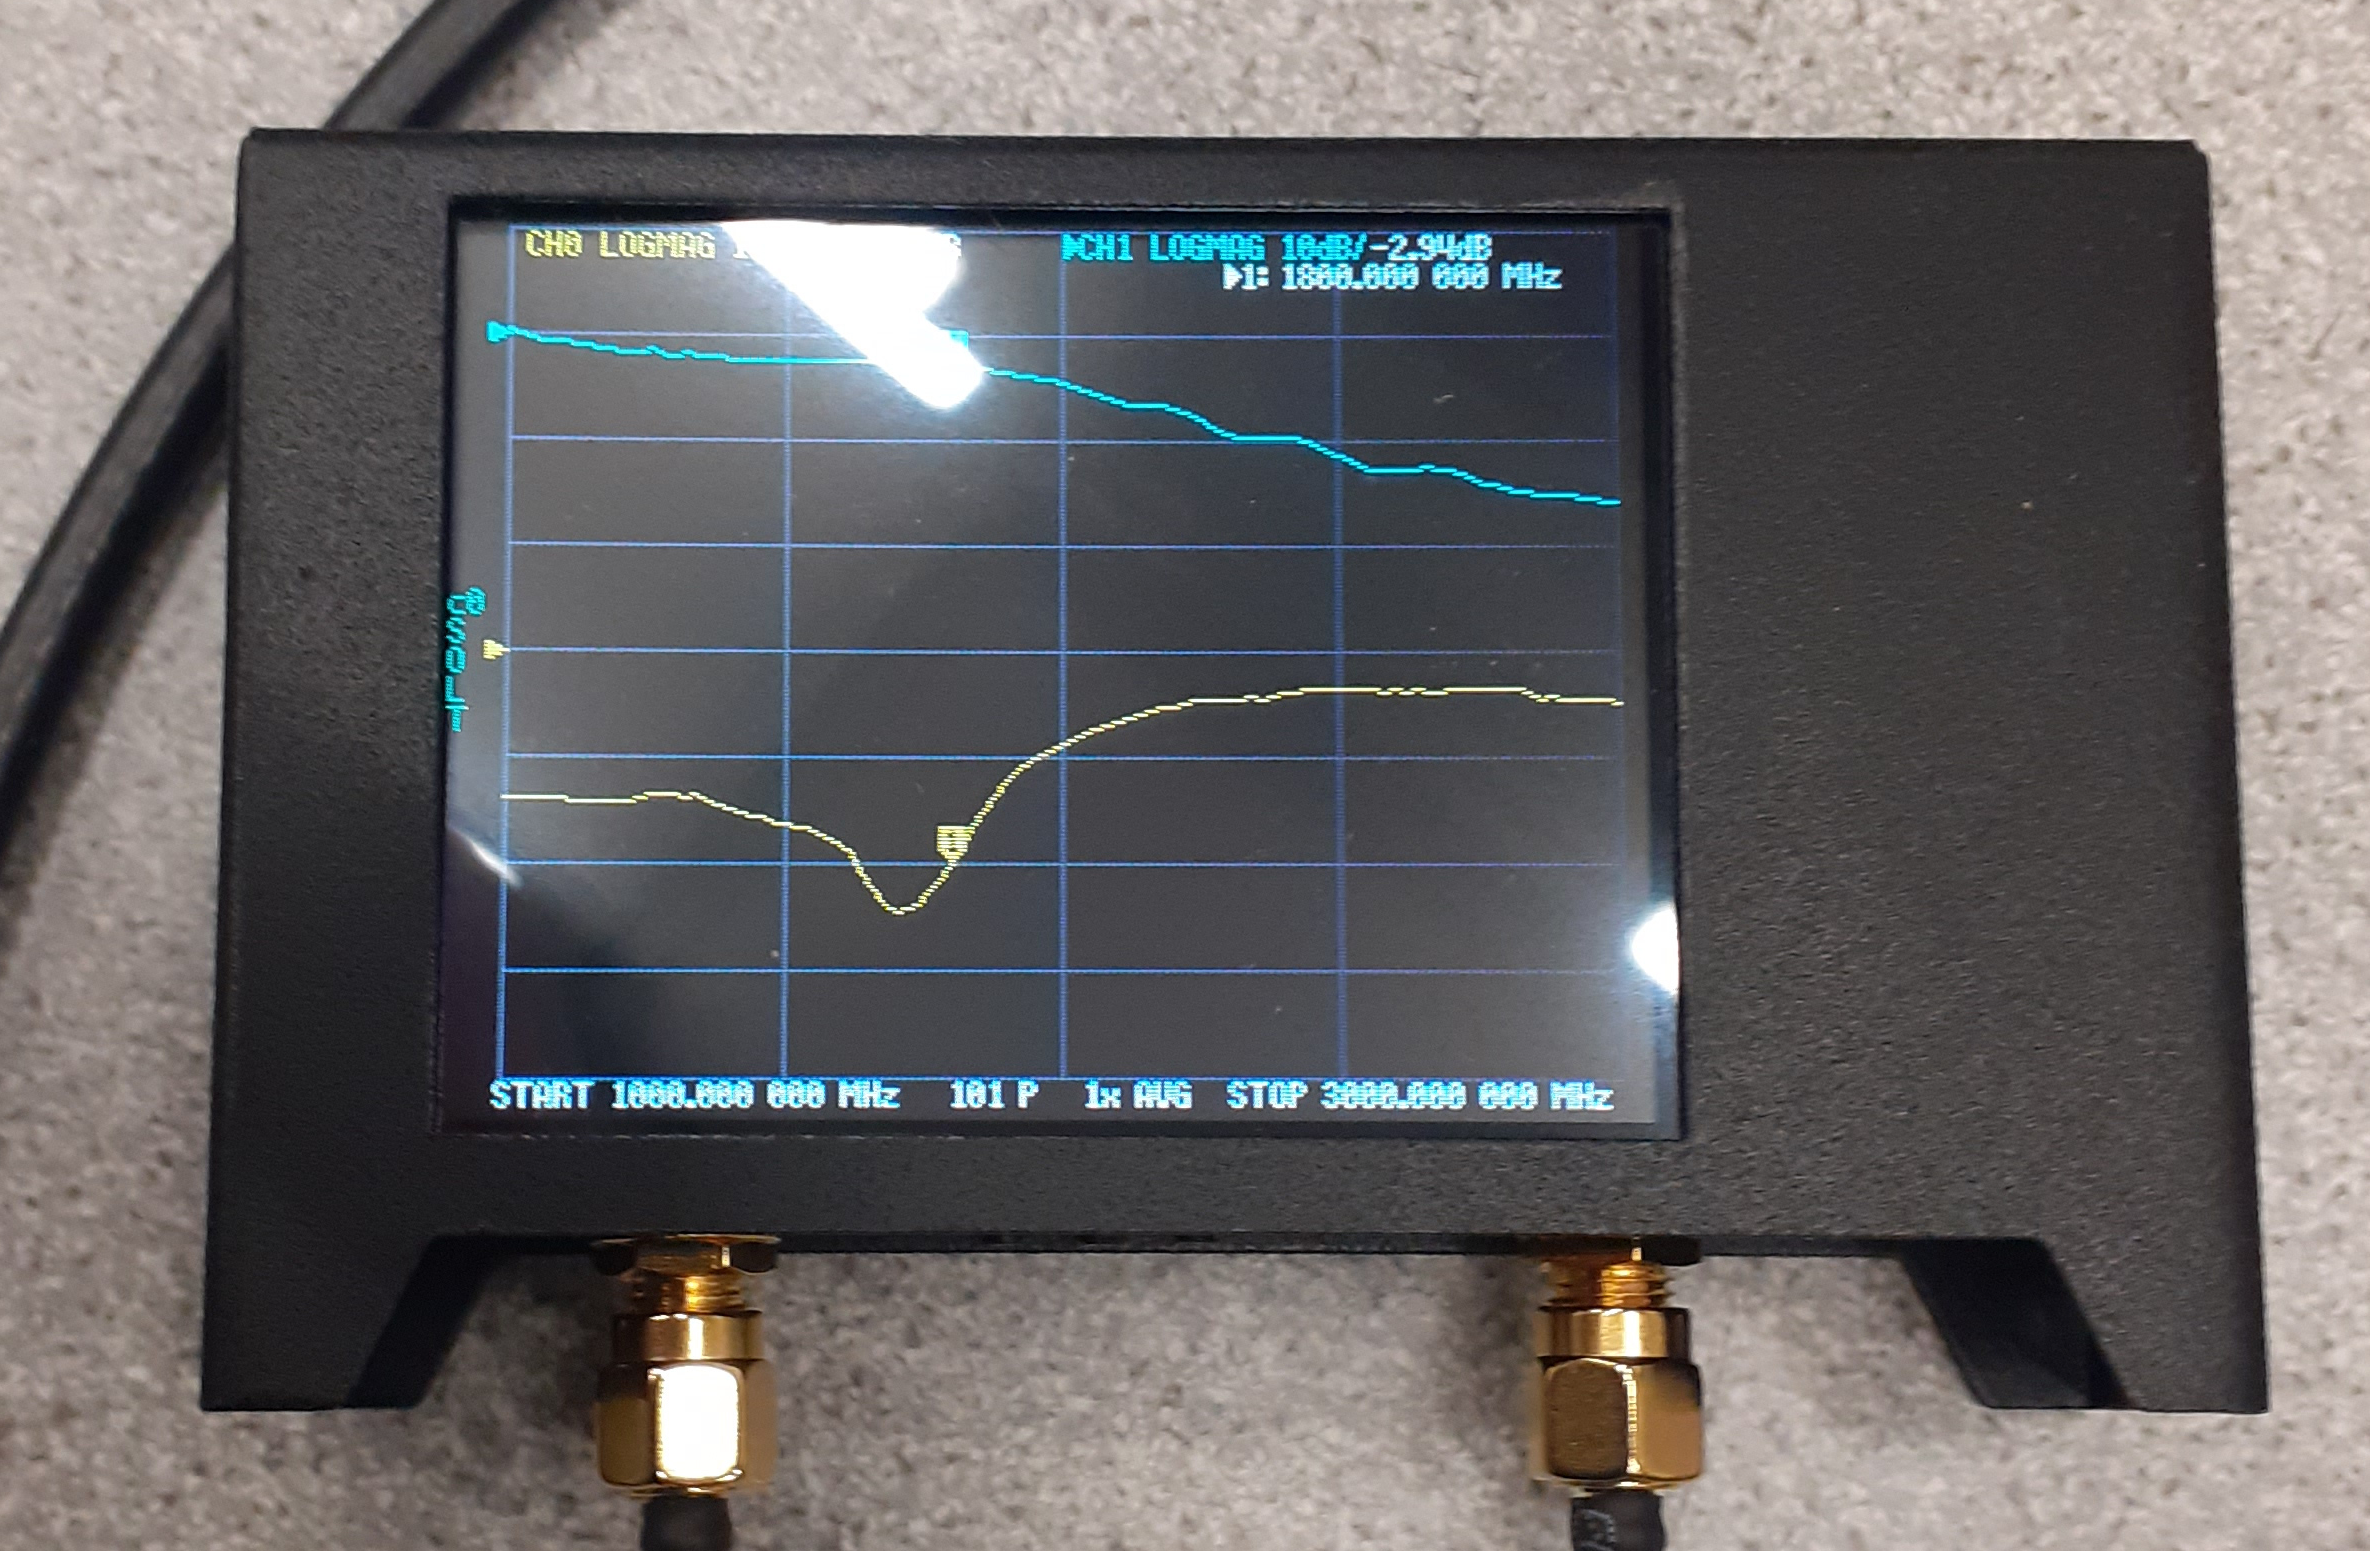
\includegraphics[scale=0.1]{photos/VNA.png}
  \caption{NanoVNA, type SAA2}
  \label{fig4}
\end{figure}
Additionally a 10 dB damper was used at the output which is visible at the following picture
which displays the base-emitter voltage at 0.7 V (bearly visible) as well as the collector-emitter
voltage where the optimal repsonse was found to be at 3.01 V, while the S-parameters used
were specified for 6 V $V_{CE}$
\begin{figure}[H]
\centering
  \includegraphics[scale=0.05]{photos/setup.png}
  \caption{Voltages sources set-ups, 10dB damper visible far down}
  \label{fig4}
\end{figure}
From the VNA display we see that $S_{21}$ is at -2.97 dB which without the 10 dB damper would be
10-2.97 = 7.03 dB ad without the two bias tees would which dampess the signal 0.4dB each
would result i an overall $S_{21}$ of 7.83 dB which is unfortuately 5.17 dB lower than specified 13 dB Gain.
This could be due to the quality of the FR4 and to the glue used to conect the copper to the
FR4 board as well as the poor accuracy of the dimensions and the placing of the copper strips because being cut
and placed manually. Additionally $S_{11}$ is seen to have a nice dip but this was not the case
in the simulation results of the LNA, see figure 36. 

\section{Conclusion}
 It seems that implementation in the physical world
 can differ quite a lot from theory. It is unclear how much of the discrepancy is due to
poor transitor quality, poor laminate quality and how much of the discrepancy is due to the uncertainties with respect to the micro strip 
dimensions and the placement of the stubs. It would also have been interesting to find out
how much the results would differ when the same transistor is used in
pcb board preapared by a milling machine. I would also really like the option of having
a socket for the transistor and try 10 different samples of the same transistor.

\section{Appendix computer code Octave}
File mstrip.m
\begin{verbatim}
\% File mstrip.m
f=1.8E+9
c=3E+8
lambda= c/f;
ko=2*pi/lambda
epsilon_r=4.4
Z0=50
d=1.6E-3

loss_tangent=0.0018


A=(Z0/60)*sqrt((epsilon_r +1)/2)+((epsilon_r-1)/(epsilon_r+1))*(0.23+0.11/epsilon_r)
B=(377*pi)/(2*Z0*sqrt(epsilon_r))

%For a given impedance Z0 and dielectric constant epsilon_r
%W/d-ratio can be found a
W2d_ratio1 =(8*exp(A))/(exp(2*A)-2)
W2d_ratio2 =(2/pi)*(B-1-log(2*B-1)+((epsilon_r-1)/(2*epsilon_r))*(log(B-1)+0.39-(0.61/epsilon_r)))
if(W2d_ratio1 <2)
 W2d_ratio = W2d_ratio1
 disp("Returned the first ratio")
elseif(W2d_ratio2 >2)
 W2d_ratio = W2d_ratio1
 disp("Returned the second ratio")
end

epsilon_eff = ((epsilon_r+1)/2)+((epsilon_r-1)/2)*(1/(sqrt(1+12*1/( W2d_ratio))))

attenuation_dielectric =(ko*epsilon_r*(epsilon_eff-1)*loss_tangent)/(2*sqrt(epsilon_eff)*(epsilon_r-1))

Width =  W2d_ratio*d


\end{verbatim}

For the LNA design
\begin{verbatim}
clear all
% addpath("/home/lasse/Documents/test M4/ewa")
i=sqrt(-1);

disp("S-Params at 1.8GHz BFG520 Common Emitter 6V10mA")
S11_r = 0.494
Theta_S11_grad=166
S21_r=3.722
Theta_S21_grad=74.3
S12_r=0.082
Theta_S12_grad= 56.4
S22_r=0.317
Theta_S22_grad= -57.9

disp("")
S=smat([0.494 166.0 3.722 74.3 0.082 56.4 0.317 -57.9 ])
disp("")


Theta_S11_rad = Theta_S11_grad*pi/180
S11 = S11_r*(cos(Theta_S11_rad)+i*sin(Theta_S11_rad))
disp("")


Theta_S21_rad=Theta_S21_grad*pi/180
S21=S21_r*(cos(Theta_S21_rad)+i*sin(Theta_S21_rad))
disp("")


Theta_S12_rad=Theta_S12_grad*pi/180
S12=S12_r*(cos(Theta_S12_rad)+i*sin(Theta_S12_rad))
disp("")



Theta_S22_rad=Theta_S22_grad*pi/180
S22=S22_r*(cos(Theta_S22_rad)+i*sin(Theta_S22_rad))

disp("")


%Stability check
disp('Stability check')
Delta = S11*S22-S12*S21
K_Stab=(1-abs(S11)^2-abs(S22)^2+abs(Delta)^2)/(2*abs(S12*S21))
Abs_Delta = abs(Delta)
if(K_Stab>1 & Abs_Delta<1)
 disp("Stability OK")
else
 disp("Stability not OK")
end

[cL,rL] = sgcirc(S,'l');
[cG,rG] = sgcirc(S,'s'); % stability circles
%[c,r] = sgcirc(S,type)
smith;
smithcir(cL, rL, 1.1, 1.5);
smithcir(cG, rG, 1.1, 1.5);
disp("")

%Maximum gain calculations
disp("Maximum gain calculations")
B1=1+abs(S11)^2-abs(S22)^2 -abs(Delta)^2
B2=1+abs(S22)^2-abs(S11)^2 -abs(Delta)^2
C1=S11 - Delta*conj(S22)
C2=S22 - Delta*conj(S11)
disp("")
[K,mu,D,B1,B2,C1,C2,D1,D2] = sparam(S)
disp("")


Gamma_S_plus  = (B1 + sqrt(B1^2 -4*abs(C1)^2) )/(2*C1);
Gamma_S_minus = (B1 - sqrt(B1^2 -4*abs(C1)^2) )/(2*C1);
if(abs(Gamma_S_plus)<1)
  Gamma_MS=Gamma_S_plus
  disp("Returned Gamma_S_plus")
else
  Gamma_MS=Gamma_S_minus
  disp("Returned Gamma_S_minus")
endif

Gamma_L_plus  = (B2 + sqrt(B2^2 -4*abs(C2)^2) )/(2*C2);
Gamma_L_minus = (B2 - sqrt(B2^2 -4*abs(C2)^2) )/(2*C2);
if(abs(Gamma_L_plus)<1)
  Gamma_ML=Gamma_L_plus
  disp("Returned Gamma_L_plus")
else
  Gamma_ML=Gamma_L_minus
  disp("Returned Gamma_L_minus")
endif


%%Absolute values of Gammas must be less than 1
disp("Absolute values of Gammas must be less than 1")



AbsGamma_MS=abs(Gamma_MS)
[THETA, R] = cart2pol (real(Gamma_MS), imag(Gamma_MS));
Theta_deg = THETA*180/pi

AbsGamma_ML=abs(Gamma_ML)
[THETA, R] = cart2pol (real(Gamma_ML), imag(Gamma_ML));
Theta_deg = THETA*180/pi
disp("")

disp("Gammas according to Matlab toolbox")
[Gamma_S_Match , Gamma_L_Match ]= smatch(S)
disp("")

%Gamma to impedances. Realpart cannot be negative
disp("Gamma to impedances. Real part cannot be negative!")
z_S =(1+Gamma_MS)/(1-Gamma_MS)
z_L=(1+Gamma_ML)/(1-Gamma_ML)
disp("Impedances from Matlab")
z_S_matlab=g2z(Gamma_MS,50)/50
z_L_matlab=g2z(Gamma_ML,50)/50
disp("Conjugated impedances are the transformation goals on Smith chart")
z_S_conj=conj(z_S)
z_L_conj=conj(z_L)



%S21 gain
disp("S21 gain")
G_0=abs(S21)^2
G_0_dB=10*log10(G_0)
disp("")

%Gains of matching networks
disp("Gains of matching networks")
G_S=1/(1-abs(Gamma_MS)^2)
G_S_dB=10*log10(G_S)
disp("")
G_L=(1-abs(Gamma_ML)^2)/(abs(1-S22*Gamma_ML)^2)
G_L_dB=10*log10(G_L)
disp("Gt gain")
Total_Gain = G_0*G_S*G_L
Total_Gain_dB = G_S_dB+G_0_dB+G_L_dB
disp("")
Gamma_L_unmatched =0;
G_power=(1/(1-abs(Gamma_MS)^2))*abs(S21)^2*((1-abs(Gamma_L_unmatched)^2)/(abs(1-S22*Gamma_L_unmatched)^2))
G_power_dB=10*log10(G_power)
Gamma_G_unmatched=0
G_availible=((1-abs(Gamma_G_unmatched)^2)/(abs(1-S11*Gamma_G_unmatched)^2))*(abs(S21)^2)*(1/(1-abs(Gamma_ML)^2))
G_availible_dB=10*log10(G_availible)



disp("Gains from toolbox")
Z0 = 50;
ZG = 50;
ZL = 50;
% normalization impedance
gG_no_matching_network = z2g(ZG,Z0);
gL_no_matching_network = z2g(ZL,Z0);
gG=Gamma_MS
gL=Gamma_ML

disp("Gamma in")
Gin = gin(S,gL)
disp("Gamma out")
Gout = gout(S,gG)%
disp("transducer power gain at given Gamma_G , Gamma_L")
Gt = sgain(S,gG,gL)
Gt_dB=10*log10(Gt)
disp("available power gain at given Gamma_G with Gamma_L = Gamma_out*")
Ga = sgain(S,gG_no_matching_network,'a')
Ga_dB=10*log10(Ga)
disp("operating power gain at given Gamma_L with Gamma_G = Gamma_in*")
Gp = sgain(S,gL_no_matching_network,'p')
Gp_dB=10*log10(Gp)
disp("maximum unilateral gain")
Gu = sgain(S,'u')
Gu_dB=10*log10(Gu)
disp("maximum available gain (MAG)")
Gmag = sgain(S)
Gmag_dB=10*log10(Gmag)
disp("maximum stable gain (MSG)")
Gmsg = sgain(S,'msg')
Gmsg_dB=10*log10(Gmsg)
%
%disp("Stubs")
%dl_in = stub1 (conj(z_S) ,'po')
%dl_out = stub1 (conj(z_L) ,'po')
%
%
%
%disp("Specific gain 13 dB")
%U=(abs(S12)*abs(S21)*abs(S11)*abs(S22))/((1-abs(S11)^2)*(1-abs(S22)^2))
%Gs_Max=1/(1-abs(S11)^2);
%Gs_Max_dB= 10*log10(Gs_Max)
%Gl_Max = 1/(1-abs(S22)^2);
%Gl_Max_dB=10*log10(Gl_Max)
%G0=abs(S21)^2;
%G0_dB=10*log(G0)
%GTU_Max = Gs_Max_dB+Gl_Max_dB+G0_dB
%%%%%%%%%%%%%%%%%%%%%%%%%%%%%%%%%%%%%%%%%%%%%%%%%
%disp("Operating power gain circles")
%[c1,r1]=sgcirc(S,'p',9)% c 1 = 0 . 4443 <52 . 56 o , r 1 = 0 . 5212
%[c2,r2]=sgcirc(S,'p',10)% c 2 = 0 . 5297 <52 . 56 o , r 2 = 0 . 4205
%[c3,r3]=sgcirc(S,'p',11.18)% c 3 = 0 . 6253 <52 . 56 o , r 3 = 0 . 2968
%[cL,rL]=sgcirc(S,'l') % c L = 2 . 0600 <52 . 56 o , r L = 0 . 9753
%smith; smithcir(cL,rL,1.7);
%% display portion of circle with |Gamma_L | <= 1 . 7
%smithcir(c1,r1);
%plot(c1,'*')
%smithcir(c2,r2);
%plot(c2,'*')
%smithcir(c3,r3);
%plot(c3,'*')
%phi = linspace(0,2*pi,361);
%gammaL = c3 + r3 * exp(j*phi);% points on 15-dB operating gain circle
%gammaG = conj(gin(S,gammaL));% circle of conjugate matched source points
%plot(gammaG);
%
%
%gL_spec = c3 - abs(r3)*exp(j*angle(c3))%GammaL closesed to the origin
%[THETA, R] = cart2pol (real(gL_spec), imag(gL_spec));
%mag_gL_spec=R
%deg_gL_spec=THETA*180/pi
%plot(gL_spec,'o')%Plot Closest Gamma_L point
%gG_match = conj(gin(S,gL_spec))%Looking into Generator should be conjugate of Gamma_in
%plot(gG_match,'x')%Plot on GammaG circle
%zL = g2z(gL_spec)
%zG = g2z(gG_match)
%dl_IN = stub1(conj(zG), 'po' )
%dl_OUT = stub1(conj(zL), 'po' )
%%%%%%%%%%%%%%%%%%%%%%%%%%%
%disp("Availible power gain circles")
%figure
%[c1,r1]=sgcirc(S,'a',11) % c 1 = 0 . 5384  < -162 . 67 o , r 1 = 0 . 4373
%[c2,r2]=sgcirc(S,'a',12) % c 2 = 0 . 6227  < -162 . 67 o , r 2 = 0 . 3422
%[c3,r3]=sgcirc(S,'a',13.2) % c 3 = 0 . 7111 <  -162 . 67 o , r 3 = 0 . 2337
%[cG,rG]=sgcirc(S,'s') % c G = 1 . 5748 <  -162 . 67 o , r G = 0 . 5162
%smith; smithcir(cG,rG,1.7);
%% plot entire source stability circle
%smithcir(c1,r1);
%plot(c1,'*')
%smithcir(c2,r2);
%plot(c2,'*')
%smithcir(c3,r3);
%plot(c3,'*');
%phi = linspace(0,2*pi,361);
%gammaG = c3 + abs(r3) * exp(j*phi);% points on 15-dB available gain circle
%gammaL = conj(gout(S,gammaG));% circle of conjugate matched loads
%plot(gammaL);
%gG_spec = c3 - abs(r3)*exp(j*angle(c3))%GammaG closesed to the origin
%plot(gG_spec,'o')%Plot Closest Gamma_L point
%gL_match = conj(gout(S,gG_spec))%Looking into Load should be conjugate of Gamma_out
%plot(gL_match,'x')%Plot on GammaL circle
%zL = g2z(gL_match)
%zG = g2z(gG_spec)
%dl_IN = stub1(conj(zG), 'po' )
%dl_OUT = stub1(conj(zL), 'po' )
%
%disp("Microstrips")
%lambda_mm=1000*3E8/1.8E9
%d=1.6E-3
%epsilon_r = 4.4
%losstangent = 0.0018
%copper_thickness = 34E-6
%u=mstripr(epsilon_r,50)
%e_eff= mstripa(epsilon_r,u)
%lambda_eff_mm =lambda_mm/sqrt(e_eff)
%Width = u*d
%stub_in_mm=dl_IN(2,1)*lambda_eff_mm
%stub_series_in_mm=dl_IN(2,2)*lambda_eff_mm
%stub_out_mm = dl_OUT(2,1)*lambda_eff_mm
%stub_series_out_mm = dl_OUT(2,2)*lambda_eff_mm

%Noise figure
disp("Noise figure calculations")
Fmin = 1.90; rn = 0.16; gGopt = p2c(0.242 ,134.0 );
%2000     1.90         .242    134.0       .160

Gmag = db(sgain(S,'mag'))% maximum available gain
Gaopt = db(sgain(S,gGopt,'a'))% available gain at Gamma_G opt
gLopt = conj(gout(S,gGopt))  % matched load

figure;
smith;
%plot([gGopt, gLopt],'x');
plot(gGopt,'*r')
plot(gLopt,'xk')
[c0,r0]=nfcirc(1.9,Fmin,rn,gGopt);
[c1,r1]=nfcirc(1.95,Fmin,rn,gGopt);
[c2,r2]=nfcirc(1.96,Fmin,rn,gGopt);
[c3,r3]=nfcirc(2.1,Fmin,rn,gGopt);
[c4,r4]=nfcirc(2.2,Fmin,rn,gGopt);
smithcir(c0,r0);
plot(c0,'*')
smithcir(c1,r1);
plot(c1,'*')
smithcir(c2,r2);
plot(c2,'*')
smithcir(c3,r3);
plot(c3,'*')
smithcir(c4,r4);
plot(c4,'*')
%Simultaneous conjugate match
[gG,gL] = smatch(S)
plot([gG,gL],'*g')
F = nfig(Fmin, rn, gGopt, gG)
phi = linspace(0,2*pi,721);
gGammas = c2 + r2*exp(j*phi);% Gamma_G around the c 2 , r 2 circle
G = db(sgain(S,gGammas,'a'));% available gain in dB
[Ga,i] = max(G) % maximum available gain
%find an index in array of a specific gain
index=1;
sizeG = 721
%for(i=1:1:sizeG)
%G(i)
% if (G(i)>13.0 ) && (G(i)<13.0)
%   index=i
%   G(i)
%   disp("found index")
%   break;
% endif
%end
gammaG = gGammas(i) % Gamma_G for maximum gain
%gammaG = gGammas(index) % Gamma_G for specific gain
gammaL = conj(gout(S,gammaG))
[ca,ra] = sgcirc(S,'a',Ga);% available gain circle
plot(ca,'*r')
smithcir(c2,r2);
smithcir(ca,ra);
plot([gammaG,gammaL],'*b');
figure
plot(phi*180/pi, G);
zG=(1+gammaG)/(1-gammaG)
zL=(1+gammaL)/(1-gammaL)
dl_IN_noiseFig = stub1 (conj(zG), 'po' )
dl_OUT_noiseFig = stub1 (conj(zL), 'po' )
disp("")

disp("Stubs T-line")
lambda_mm=1000*3E8/1.8E9
stub_in_mm = dl_IN_noiseFig(2,1)*lambda_mm
serial_in_mm=dl_IN_noiseFig(2,2)*lambda_mm

stub_out_mm = dl_OUT_noiseFig(2,1)*lambda_mm
serial_out_mm=dl_OUT_noiseFig(2,2)*lambda_mm
disp("")

disp("Microstrips")
d=1.6E-3
epsilon_r = 4.4
losstangent = 0.0018
copper_thickness = 34E-6
u=mstripr(epsilon_r,50)
e_eff= mstripa(epsilon_r,u)

lambda_eff_mm =lambda_mm/sqrt(e_eff)
Width = u*d

stub_in_mm = dl_IN_noiseFig(2,1)*lambda_eff_mm
serial_in_mm=dl_IN_noiseFig(2,2)*lambda_eff_mm

stub_out_mm = dl_OUT_noiseFig(2,1)*lambda_eff_mm
serial_out_mm=dl_OUT_noiseFig(2,2)*lambda_eff_mm

\end{verbatim}

\end{document}
\vfill\null
\clearpage
\columnbreak
\newpage


%pdflatex --shell-escape testQ.tex